\chapter{Strings}

\section{ Z-string function and its calculation } % Revisado por MGP
Let a string $s$ of length $n$. Then the \textbf{Z-function} of this string is an array of length $n$, $i$-th element of which is equal to the greatest number of characters starting from the position $i$ coinciding with the first characters from $s$. In other words, $z [i]$ is the greatest common prefix of $s[0..n-1]$ and $s[i..n-1]$.

\textbf{Note.} In this paper, to avoid ambiguity, we assume that the string is 0-indexed - that is, the first character has an index of $0$, And the last is $n-1$.

The first element of Z-function $z [0]$ is generally considered undefined. In this article, we will assume that it is zero (although this is not always the case, this does not change anything).

This article provides an algorithm for computing the Z-function in time $O (n)$ as well as various applications of the algorithm.

\subsection{ Examples }

$" aaaaa"$ :
$z [0] = 0;$
$z [1] = 4;$
$z [2] = 3;$
$z [3] = 2;$
$z [4] = 1.$

$" aaabaab"$ :
$z [0] = 0;$
$z [1] = 2;$
$z [2] = 1;$
$z [3] = 0;$
$z [4] = 2;$
$z [5] = 1;$
$z [6] = 0.$

$" abacaba"$ :
$z [0] = 0;$
$z [1] = 0;$
$z [2] = 1;$
$z [3] = 0;$
$z [4] = 3;$
$z [5] = 0;$
$z [6] = 1.$

\subsection{ Trivial algorithm }

The formal definition can be expressed as the following elementary implementation in $O (n ^ 2)$:

\begin{verbatim}
vector < int > z_function_trivial(string s){
    int n =(int)s. length() ;
    vector < int > z(n);
    for(int i = 1 ; i < n ; ++ i )
        while(i + z[i]< n && s[z[i]] == s[i + z[i]] )
            ++ z[i];
    return z ;
} 
\end{verbatim}
We just iterate each position $i$ to sort out the answer to it, $z [i]$. Starting from zero, we increment $z[i]$ as long as we do not detect a mismatch or get to the end of the string.

Of course, this version is too inefficient, we now turn to the construction of an efficient algorithm.

\subsection{ An efficient algorithm for computing the Z-function }

to obtain an efficient algorithm, we calculate the values $z [i]$ one at a time - from $i = 1$ to $n-1$. And at the same time we try to calculate the next value $z [i]$ with maximum use of already computed values.

We call a substring that matches the prefix $s$, a \textbf{segment}. For example, the value of the desired Z-function $z [i]$ is the longest segment starting at position $i$ (and it will end at position $i + z [i] - 1$).

To do this, we will keep \textbf{an interval} \textbf{$[l; r]$} \textbf{of the rightmost matched segment}, i.e, of all detected segments will keep the one that ends rightmost. In a sense, the index $r$ is the current boundary which our string has been scanned by the algorithm and all the rest are not yet known.

Then, if the current index for which we want to calculate the next value of Z-function is $i$, We have one of two options:

$i> r$ - That is, current position \textbf{is after} of what we have already treated.
Then we will calculate $z [i]$ using the \textbf{trivial algorithm}, i.e, just trying values $z [i] = 0$, $z [i] = 1$, etc. Note that in the end, if $z [i]$ is $> 0$ then we will have to update the position of the rightmost segment $[l; r]$ because $i + z [i] - 1$ is guaranteed to be more than $r$.

$i \le r$ - That is, current position is inside the rightmost segment $[l; r]$.
Then we can use the already calculated values ​​of \textbf{the previous} Z-function to initialize the value of $z [i]$ greater than zero.

For this we note that the substring $s [l \ldots r]$ and $s [0 \ldots r-l]$ \textbf{coincide}. This means that, as an initial lower bound for $z [i]$ we can take the corresponding value of the segment $s [0 \ldots r-l]$, namely, the value of $z [i-l]$.

However, the value $z [i-l]$ might be too much, so that when it is applied to the position $i$ it gets out of the boundary $r$. This can not be allowed, since we know nothing about the characters to the right of $r$.

Here is an \textbf{example} of such a situation:

$" aaaabaa" $

When we get to the last position ($i = 6$), the current right-most segment is $[5, 6]$. Position $6$ using this segment will match the position $6-5 = 1$, which answer  is $z [1] = 3$. Obviously, such a value to initialize $z [6]$ is impossible. The maximum value we can initialize is $1$ because it is the largest value that is not beyond the interval $[l; r]$.

Thus, as an \textbf{initial lower bound} for $z [i]$ it is safe to take the expression:

$z_0 [i] = \min (r-i +1, z [i-l])$

Thus, the whole algorithm has two cases that differ only in \textbf{the initial value} of $z [i]$. In the first case, it is assumed to be zero and the second, it is determined by the previous value at the specified formula. After that, the two branches of the algorithm are reduced to \textbf{a trivial string matching algorithm}  with the specified initial value.

The algorithm turned out to be quite simple. Despite the fact that for each $i$ it runs the trivial algorithm - this is significantly better, having an algorithm that runs in linear time. To see why this is so, consider the discussion after the implementation of the present algorithm.

\subsection{ Implementation }

Implementation turns out rather succinct:

\begin{verbatim}
vector < int > z_function(string s){
    int n =(int)s. length() ;
    vector < int > z(n);
    for(int i = 1, l = 0, r = 0 ; i < n ; ++ i){
        if(i <= r )
            z[i]= min(r - i + 1, z[i - l ]);
        while(i + z[i]< n && s[z[i]] == s[i + z[i]] )
            ++ z[i];
        if(i + z[i]- 1 > r )
            l = i,  r = i + z[i]- 1 ;
    }
    return z ;
} 
\end{verbatim}

\subsection{Comment on this implementation}

The whole solution is given as a function that returns an array of length $n$, the Z-function itself.

Array $z []$ is initially filled with zeros. The current rightmost segment is assumed to match $[0, 0]$, i.e, a deliberate small segment, which will not include any $i$.

Inside the loop with $i = 1 \ldots n-1$ we first determine the initial value of $z [i]$ - it will be either zero or calculated based on the above formula.

After that, we have the trivial algorithm that attempts to increase the $z [i]$ as much as possible.

Then, we update the current segment of the rightmost match $[l; r]$ if this update is required - i.e. if $i + z [i] -1> r$.

\subsection{ Asymptotic behavior of the algorithm }

We prove that the above algorithm runs in linear time with respect to the string length, i.e. $O (n)$.

The proof is very simple.

We are interested in the nested $\rm while$ loop, because in everything else only constant operations are performed $O (n)$ times.

We show that \textbf{each iteration} of the $\rm while$ loop increases the right border $r$ by one.

For this, consider the two branches of the algorithm:

$i> r$
In this case, either the $\rm while$ cycle will not make a single iteration (if $s [0] \ne s [i]$)or it will make a few iterations, each time moving one character to the right, starting at $i$. And after that the right border $r$ is surely updated.

Since $i> r$, we find that indeed, each iteration of the cycle increases the value $r$ by one.

$i \le r$
In this case, we initialize the value of the above formula $z [i]$ with a certain number $z_0$. Compare this initial value $z_0$ with the value $r-i +1$, we have three options:

$z_0 <r-i +1$
We prove that in this case the $\rm while$ loop will not iterate.

This is easy to prove for example, on the contrary. If the $\rm while$ loop made at least one iteration, it would mean that $z_0$ we have defined value was not accurate, because it is less the length of this match. But since string $s [l \ldots r]$ and $s [0 \ldots r-l]$ match, it means that the position $z[i-l]$ is an invalid value - less than it should be.

Thus, supposing the correct value $z [i-l]$ and the fact that it is less $r-i +1$, it follows that this value coincides with the desired value $z [i]$.

$z_0 = r-i +1$
In this case the $\rm while$ loop can perform several iterations, but each of them will increase the value of the new $r$ by one, because the first character being compared is $s [r +1]$ which resides beyond the interval $[l; r]$.

$z_0> r-i +1$
This option is not possible in principle, by the definition of $z_0$.

Thus, we have proved that each iteration results in a nested loop to move the pointer $r$ to the right. Because $r$ cannot be greater than $n-1$, this means that this loop will not perform more than $n-1$ iterations total.

As the rest of the algorithm obviously works in $O (n)$, then we have proved that the whole algorithm Z-function runs in linear time.

\subsection{ Applications }

We consider several applications Z-functions for specific tasks. These applications will be largely similar to using a prefix function.

\subsubsection{ String search }

To avoid confusion, we call one string a \textbf{text} $t$ and the other a \textbf{pattern} $p$. Thus, the task is to find all occurrences of the pattern $p$ in the text $t$.

To solve this problem, we form a string $s = p + \# + t$, i.e, concatenate the text to the pattern through a separator character (which is not found anywhere in the strings themselves).

Calculate the resulting Z-line function. Then for any $i$ in the interval $[0; length (t) -1]$, by the corresponding value $z [i + length (p) + 1]$ you can test whether the sample $p$ is in the text $t$ beginning at position $i$: if this Z-function value is equal to $length (p)$, then yes, otherwise no.

Thus, the asymptotic behavior of the solution is $O(length (t) + length (p))$. Memory consumption has the same asymptotics.

\subsubsection{ Number of distinct substrings in a string }

Given a string $s$ length $n$ we need to count the number of its different substrings.

We solve this problem iteratively. Specifically, knowing the current number of distinct substrings we recalculate the number when adding one character to the end of the string.

So, let $k$ be the current number of different substrings in $s$ and we append the character $c$. Obviously, we have some new substrings ending in this new character $c$ (that is, all the strings that end with this character, but never met before).

Take string $t = s + c$ and reverse it. Our task is to count how many prefixes of $t$ are not found anywhere else in it. But if we calculate the Z-function of string $t$ and find its maximum value $z_ {\rm max}$, then, obviously, in the string $t$ occurs (not leading) the prefix length $z_ {\rm max}$ but no longer. Clearly, shorter prefixes also occurs.

So, we found that the number of new substrings that appear when appending character $c$ is $len - z_ {\rm max}$, where $len$ is the current length of the string after appending the character $c$.

Consequently, the solution's asymptotic time for a string of length $n$ is $O (n ^ 2)$.

It should be noted that exactly the same can be recalculated for $O (n)$ the number of different substrings and append a character to the top, as well as removing a character from the end or the beginning.

\subsubsection{ Row compression }

Given a string $s$ of length $n$. It is required to find its shortest "compressed" representation, i.e, find a string $t$ of minimum length such that $s$ can be represented as a concatenation of one or more copies of $t$.

To obtain the solution, calculate the Z-function of $s$ and find the first position $i$ such that $i + z [i] = n$. Then, the string $s$ can be compressed to a string of length $i$.

The proof of such a decision does not differ from the solution with the prefix function.

\subsection{ Tasks in the online judges }

List of tasks that can be solved using the Z-function:
\begin{itemize}
\item UVA 455 \textbf{"Periodic Strings"} [Difficulty: Medium]
\item UVA 11022 \textbf{"String Factoring"} [Difficulty: Medium]
\end{itemize}

\section{ Prefix function and Knuth-Morris-Pratt algorithm } % Parcialmente revisado por MGP
\subsection{ Prefix function definition }

Given a string $s [0 \ldots n-1]$ we calculate its prefix function, i.e, an array of numbers $\pi [0 \ldots n-1]$, where $\pi [i]$ is defined as follows: it is the length of the longest proper suffix in substring $s [0 \ldots i]$ coinciding with its prefix (proper suffix - so not the entire string). In particular, the value $\pi [0]$ is set equal to zero.

The mathematical definition of the prefix function can be written as follows:

$\pi[i]=\underset{k=0\ldots i}{\max}\{k:s[0\ldots k-1]=s[i-k+1\ldots i]\}$

For example, the string "abcabcd" prefix function is: $[0, 0, 0, 1, 2, 3, 0]$, which means:

For "a" the trivial prefix matches the suffix;
For "ab" the trivial prefix matches the suffix;
For "abc" the trivial prefix matches the suffix;
For "abca" prefix of length $1$ coincides with the suffix;
For "abcab" prefix of length $2$ coincides with the suffix;
For "abcabc" prefix of length $3$ coincides with the suffix;
For "abcabcd" the trivial prefix matches the suffix.

Another example: for string "aabaaab" it is equal to: $[0, 1, 0, 1, 2, 2, 3]$.

\subsection{ Trivial algorithm }

Immediately following the definition, we can write the following algorithm for computing the prefix function:

\begin{verbatim}
vector < int > prefix_function(string s){
    int n =(int)s. length() ;
    vector < int > pi(n);
    for(int i = 0 ; i < n ; ++ i )
        for(int k = 0 ; k <= i ; ++ k )
            if(s. substr(0,k)== s. substr(i - k + 1,k))
                pi[i]= k ;
    return pi ;
} 
\end{verbatim}
As you can see, it will work in $O (n ^ 3)$ which is too slow.

\subsection{ An efficient algorithm }

This algorithm was developed by Knuth and Pratt and independently by Morris in 1977 (as a basic element for the search algorithm of a string).

\subsubsection{ The first optimization }

The first important point is that the value of $\pi [i +1]$ does not exceed more than one unit the value $\pi [i]$ for any $i$.

Indeed, otherwise if $\pi [i +1]> \pi [i] + 1$ then consider this suffix ending at position $i +1$ and of length $\pi [i +1]$. By removing the last character, we obtain a suffix ending at position $i$ and of length $\pi [i +1] -1$, which is a better $\pi [i]$, i.e, a contradiction. An illustration of this conflict (in this example $\pi [i-1]$ should be equal to 3):

$\underbrace {\overbrace {s_0 s_1} ^ {\pi [i-1] = 2} s_2 s_3} _ {\pi [i] = 4} \ldots    \underbrace{s_{i-3}\overbrace {s_{i-2} s_{i-1}} ^ {\pi [i-1] = 2} s_i}  _ {\pi [i] = 4}$

(In this diagram the upper braces denote two identical substrings of length 2, and the lower braces two identical substrings of length 4)

Thus, the transition to the next element of the prefix function could either increase by one, do not change or decrease by any amount. This fact allows us to reduce the asymptotic to $O (n ^ 2)$. As in a single step the value can rise a maximum of one, the total for the entire string could occur up to $n$ increases by one, and as a result (because the value could never be less than zero), the maximum of $n$ reductions. That will have $O (n)$ string comparisons, so we have reached asymptotic $O (n ^ 2)$.

\subsubsection{ The second optimization }

Come on, \textbf{get rid of the obvious comparisons of substrings}. To do this, try to maximize the information calculated in the previous steps.

Thus, suppose we have calculated the value of the prefix function $\pi [i]$ for some $i$. Now, if $s [i +1] = s [\pi [i]]$, we can say that certainly $\pi [i +1] = \pi [i] + 1$. Illustration:

$\underbrace {\overbrace {s_0 s_1 s_2} ^ {\pi [i]} \overbrace {s_3} ^ {s_3 = s_{i+1}}} _ {\pi [i+1] = \pi[i]+1} \ldots    \underbrace{\overbrace {s_{i-2} s_{i-1} s_i} ^ {\pi [i]}  \overbrace{s_{i+1}} ^ {s_3 = s_{i+1}}} _ {\pi [i+1] = \pi[i]+1}$

Now suppose that, on the contrary, it happens that $s [i +1] \ne s [\pi [i]]$. Then we need to try a shorter substring. In order to optimize, we would like to go directly to a (maximum) length $j <\pi [i]$ that still holds the prefix property in the position $i$, i.e. $s [0 \ldots j-1] = s [i-j +1 \ldots i]$:

$\underbrace {\overbrace {s_0 s_1} ^ {j} s_2 s_3} _ {\pi [i]} \ldots    \underbrace{s_{i-3} s_{i-2} \overbrace {s_{i-1} s_i} ^ {j}}  _ {\pi [i]} s_{i+1}$

Indeed, when we find such a length $j$, again will be sufficient to compare the characters $s [i +1]$ and $s [j]$. If they match, it can be argued that $\pi [i +1] = j +1$. Otherwise, we need to re-find a smaller (the next largest) value $j$ for which the prefix property, and so on. It may happen that these values $j$ run out - this happens when $j = 0$. In this case, if $s [i +1] = s [0]$, then $\pi [i +1] = 1$, otherwise $\pi [i +1] = 0$.

Thus, we already have the general scheme of the algorithm, there is only the unresolved issue of finding $j$ effectively. We pose this question formally, for the current length $j$ and positions $i$ (for which the prefix property holds, i.e. $s [0 \ldots j-1] = s [i-j +1 \ldots i]$). It is required to find the greatest $k <j$ for which still holds the prefix property:

$\underbrace {\overbrace {s_0 s_1} ^ {k} s_2 s_3} _ {j} \ldots    \underbrace{s_{i-3} s_{i-2} \overbrace {s_{i-1} s_i} ^ {k}}  _ {j} s_{i+1}$

After such a detailed description it practically begs that this value $k$ is none other than the value of the prefix function $\pi [j-1]$ which has already been evaluated previously (subtraction by one comes from the 0-indexed strings). Thus, to find the length $k$ we can do in $O (1)$ each.

\subsubsection{ The final algorithm }

So, we finally constructed an algorithm that does not contain explicit string comparisons and performs in $O (n)$.

We present here the final scheme of the algorithm:

Calculate the values ​​of the prefix function $\pi [i]$ in order, from $i = 1$ to $i = n-1$ (for value $\pi [0]$ simply assign zero).
To calculate the current value $\pi [i]$ we lead the variable $j$ for the length of the current prefix. Initially $j = \pi [i-1]$.
Test a prefix of length $j$, comparing the characters $s [j]$ and $s [i]$. If they are the same then we set $\pi [i] = j +1$ and proceed to the next index $i +1$. If the symbols are different, we decrease the length of $j$ by setting it equal to $\pi [j-1]$ and repeat this step of the algorithm from the beginning.
If we come to a length $j = 0$ and did not find a match it will stop the process and set $\pi [i] = 0$ and proceed to the next index $i +1$.
\subsubsection{ Implementation }

Algorithm eventually turned remarkably simple and concise:

\begin{verbatim}
vector < int > prefix_function(string s){
    int n =(int)s. length() ;
    vector < int > pi(n);
    for(int i = 1 ; i < n ; ++ i){
        int j = pi[i - 1];
        while(j > 0 && s[i]! = s[j])
            j = pi[j - 1];
        if(s[i]== s[j ]) ++ j ;
        pi[i]= j ;
    }
    return pi ;
} 
\end{verbatim}
As you can see, the algorithm is an \textbf{online} algorithm, i.e. it processes the data in the course of receipt - you can, for example, read the string one character at once to handle this character, finding the answer to the next position. The algorithm requires storage of the string itself and the previous calculated values of ​​prefix function, but it is easy to see that if we know in advance the maximum value that can take the prefix on the entire string, it will be sufficient to keep only one more than the number of the first character and values prefix function.
%???

\subsection{ Applications }

\subsubsection{ Search for substring }

This problem is a classic use of the prefix functions (and, in fact, they were discovered in this application).

Given text $t$ and a string $s$, find and display the positions of all occurrences of the string $s$ in the text $t$.

For convenience let $n$ be the length of string $s$ and $m$ the length of the text $t$.

We form a string $s + \# + t$, where the symbol $\#$ is a separator, which should not occur anywhere else. Calculate the prefix function for this string. Now consider its meaning, but only the first $n +1$ positions (which, as you can see, belong to the line $s$ and separator). By definition, the value of $\pi [i]$ shows naidlinneyshuyu length substring ending at position $i$ and coincides with a prefix. But in this case, $\pi [i]$ - The actual length of the largest block matching with a string $s$ and ending at position $i$. More than $n$, This length can not be - through the separator. But equality $\pi [i] = n$ (Where it is reached), means that the position $i$ ends desired occurrence of the string $s$ (Just do not forget that all positions are measured in line glued $s + \# + t$ ).

Thus, if at any position $i$ was $\pi [i] = n$, The position $i - (n + 1) - n + 1 = i - 2 n$ line $t$ begins the next occurrence of the string $s$ in line $t$.

As mentioned in the description of the algorithm for calculating the prefix function, if it is known that the values ​​of the prefix functions will not exceed a certain value, it is sufficient to store a whole string and prefix function, but only the beginning. In our case, this means that you need to keep in mind a line $s + \#$ and the value of the prefix function on it, and then read one character string $t$ and recalculate the current value of the prefix function.

Thus, the algorithm is the Knuth-Morris-Pratt solves this problem for $O (n + m)$ time and $O (n)$ memory.

\subsubsection{ Counting the number of occurrences of each prefix }

Here we consider two problems at once. Given a string $s$ length $n$. The first option is required for each prefix $s [0 \ldots i]$ count how many times it occurs in the very same line $s$. In the second version of the problem is given another row $t$, And is required for each prefix $s [0 \ldots i]$ count how many times it occurs in $t$.

We solve the first problem first. Cover in any position $i$ value prefix function in it $\pi [i]$. By definition, it means that the position $i$ ending prefix of entry $s$ length $\pi [i]$ And no longer end up in the position of the prefix $i$ can not. At the same time, in the position $i$ could end up, and the occurrence of prefixes shorter lengths (and, obviously, not necessarily the length of $\pi [i] -1$ ). However, it is easy to see, we have come to the same question, to which we have already met in the consideration of an algorithm to compute the prefix function: for a given length $j$ I must say, what naidlinneyshy its own suffix coincides with the prefix. We found out that the answer to this question will be $\pi [j-1]$. But then in this problem, if the position $i$ occurrence of a substring ends length $\pi [i]$ Coinciding with the prefix, the $i$ also ends occurrence of a substring of length $\pi [\pi [i] -1]$ Coinciding with the prefix, but for her the same arguments apply, so $i$ also ends, and the occurrence of length $\pi [\pi [\pi [i] -1] -1]$ and so on (as long as the index does not become zero.) Thus, to compute the answer, we have to do this cycle:

\begin{verbatim}
vector < int > ans(n + 1);
for(int i = 0 ; i < n ; ++ i )
    ++ ans[pi[i]] ;
for(int i = n - 1 ; i > 0 ; -- i )
    ans[pi[i - 1]] + = ans[i]; 
\end{verbatim}
Here, for each value of the prefix function first count how many times he had met in an array $\pi []$ And then considered a somewhat dynamic: if we know that the prefix length $i$ Match exactly ${\rm ans} [i]$ times, it is necessary to add to the number of occurrences of its longest proper suffix that matches its prefix, then this is a suffix (of course, less than $i$ length) Run "bouncing" of the amount of your suffix, etc.

Now consider the second problem. Using the standard method: we assign to the line $s$ line $t$ delimited, i.e. Given a string $s + \# + t$ And considered it to prefix function. The only difference from the first task will be that it is necessary to consider only those values ​​prefix functions that belong to the line $t$ i.e. all $\pi [i]$ for $i \ge n +1$.

\subsubsection{ Number of distinct substrings in a string }

Given a string $s$ length $n$. Need to count the number of its different substrings.

We solve this problem iteratively. Specifically, learn, knowing the current number of distinct substrings, recalculate the number when added to the end of one character.

So, let $k$ - The current number of different substrings $s$ And we append the symbol $c$. Obviously, due to some new substring ending in this new symbol $c$. Namely, added as new ones substring ending in symbol $c$ not seen before.

Take line $t = s + c$ and invert it (write the characters in reverse order). Our task - to count how many rows $t$ these prefixes that are not found anywhere else in it. But if we believe the string $t$ prefix function and find its maximum value $\pi_ {\rm max}$ Then, obviously, in the line $t$ occurs (not leading) the prefix length $\pi_ {\rm max}$ But no longer. Clearly, prefixes shorter certainly found it.

So, we found that the number of new substrings that appear when appending characters $c$ Well $s. {\rm length}() + 1 - \pi_ {\rm max}$.

Thus, for each character we are for Append $O (n)$ can count the number of different substrings. Consequently, for the $O (n ^ 2)$ we can find a number of different substrings for any given line.

It should be noted that exactly the same you can count the number of different substrings and append a character to the top, as well as removing a character from the end or the beginning.

\subsubsection{ Row compression }

Given a string $s$ length $n$. Required to find the shortest of its "compressed" representation, i.e. Find this line $t$ minimum length that $s$ can be represented as a concatenation of one or more copies $t$.

It is clear that the problem is to find the length of the string $t$. Knowing the length of the answer to the problem will, for example, the prefix string $s$ this length.

Count on the line $s$ prefix function. Consider its last value, i.e. $\pi [n-1]$, And introduce the notation $k = n - \pi [n-1]$. We show that if $n$ divided by $k$, It $k$ and will be a long answer, otherwise effective compression does not exist, and the answer is $n$.

In fact, let $n$ divided by $k$. Then the line can be represented as a series of blocks of length $k$, And, by definition, the prefix function, the prefix length $n-k$ will match it with the. But then the last block must be the same as the penultimate penultimate - with predpredposlednim, etc. In the end, it turns out that all the units are the same units, and such $k$ really fit the answer.

We show that this response is optimal. Indeed, otherwise, if we had a smaller $k$, Then the prefix is ​​a function on the end would be more than $n-k$ i.e. a contradiction.

Now let $n$ is not divisible by $k$. We show that this implies that the length of the response is $n$. Prove by contradiction - assuming that the answer exists, and has a length $p$($p$ divider $n$ ). Note that the prefix function must be more $n - p$ i.e. This suffix should partially cover the first block. Now consider the second block row; as prefix matches the suffix and a prefix and suffix cover the block, and their displacement relative to each other $k$ does not divide the length of the block $p$ (Otherwise, it would $k$ divided the $n$ ), All the characters are the same block. But then, the line consists of the same character, it $k = 1$, And the answer should be, that is, so we get a contradiction.

$\overbrace{s_{0}s_{1}s_{2}s_{3}}^{p}\overbrace{s_{4}s_{5}s_{6}s_{7}}^{p}$

$s_{0}s_{1}s_{2}\underbrace{\overbrace{s_{3}s_{4}s_{5}s_{6}}^{p}s_{7}}_{\pi[7]=5}$

$s_{4}=s_{3},\, s_{5}=s_{4},\, s_{6}=s_{5},\, s_{7}=s_{6}\quad\Rightarrow\quad s_{0}=s_{1}=s_{2}=s_{3}$

\subsubsection{ Construction of automaton by the prefix function }

Let us return to that used repeatedly receive concatenate two strings delimited, i.e. data lines $s$ and $t$ prefix computation function for strings $s + \# + t$. Obviously, because symbol $\#$ is the separator, the value of the prefix function will never exceed $s. {\rm length}()$. It follows that, as mentioned in the description of the algorithm for calculating the prefix function, just enough to keep the line $s + \#$ and the values ​​of the prefix function for her, and for all subsequent characters to prefix function to calculate on the fly:

$\underbrace{s_{0}s_{1}\ldots s_{n-1}\#}_{{\rm need}\,{\rm to}\,{\rm save}}\underbrace{t_{0}t_{1}\ldots t_{m-1}}_{{\rm need}\,{\rm not}\,{\rm to}\,{\rm save}}$

Indeed, in such situations, knowing the next character $c \in t$ prefix and the value function in the previous position, it will be possible to calculate the new value of the prefix function does is not using all the previous characters of the string $t$ and the values ​​of the prefix function in them.

In other words, we can construct an \textbf{automaton:} the state it would be the current value of the prefix function, the transitions from one state to another will take place by the symbol:

$s_{0}s_{1}\ldots s_{n-1}\#\underbrace{\ldots}_{\pi[i-1]}\Rightarrow s_{0}s_{1}\ldots s_{n-1}\#\underbrace{\ldots}_{\pi[i-1]}+t_{i}\Rightarrow s_{0}s_{1}\ldots s_{n-1}\#\ldots\underbrace{t_{i}}_{\pi[i]}$

Thus, even with no strings $t$ We can pre-build a jump table $({\rm old} \_ \pi, c) \rightarrow {\rm new} \_ \pi$ using the same algorithm for computing the prefix function:

\begin{verbatim}
string s ; // input string
const int alphabet = 256 ; // output alphabet of symbols, usually less
 
s + = '#' ;
int n =(int)s. length() ;
vector < int > pi = prefix_function(s);
vector < vector < int > > aut(n, vector < int >(alphabet)) ;
for(int i = 0 ; i < n ; ++ i )
    for(char c = 0 ; c < alphabet ; ++ c){
        int j = i ;
        while(j > 0 && c ! = s[j])
            j = pi[j - 1];
        if(c == s[j ]) ++ j ;
        aut[i ][ c]= j ;
    } 
\end{verbatim}
However, in this form, the algorithm will work for $O (n ^ 2 k)$($k$ - Power of the alphabet). But note that, instead of the inner loop $\rm while$ Which gradually shortens response, we can use the already computed part of the table: the transition from the value $j$ to the value $\pi [j-1]$ We actually say that the transition from state $(J, c)$ will lead to the same state as the transition $(\pi [j-1], c)$ And for him the answer is already counted accurately (as $\pi [j-1] <j$ )

\begin{verbatim}
string s ; // input string
const int alphabet = 256 ; // output alphabet of symbols, usually less
 
s + = '#' ;
int n =(int)s. length() ;
vector < int > pi = prefix_function(s);
vector < vector < int > > aut(n, vector < int >(alphabet)) ;
for(int i = 0 ; i < n ; ++ i )
    for(char c = 0 ; c < alphabet ; ++ c )
        if(i > 0 && c ! = s[i])
            aut[i ][ c]= aut[pi[i - 1]][ c];
        else
            aut[i ][ c]= i +(c == s[i ]); 
\end{verbatim}
The result was a very simple implementation of the construction of the machine, working for $O (n k)$.

When it can be useful to such a machine? For a start let us recall that we consider the prefix function for strings $s + \# + t$, And its value is typically used for the sole purpose: to find all occurrences of the string $s$ in line $t$.

Therefore, the most obvious benefit from the construction of the automaton - \textbf{the acceleration of the prefix function} for strings $s + \# + t$. By building on the line $s + \#$ automatic, we no longer need any line $s$ Or prefix value function in it, do not need and no calculations - all transitions (i.e. how will change the prefix function) predposchitany already in the table.

But there is another, less obvious use. This is the case when the line $t$ \textbf{is a giant string, built by any rule.} This could be, for example, Gray Line or string formed recursive combination of several short lines, applied to the input.

Suppose, for definiteness, we solve \textbf{the following problem:} given a number $k \le 10 ^ 5$ Gray line, and given a string $s$ length $n \le 10 ^ 5$. Need to count the number of occurrences of the string $s$ in $k$ The second line of Gray. Recall Gray lines are defined as follows:

$g_1 =" a" $

$g_2 =" aba" $

$g_3 =" abacaba" $

$g_4 =" abacabadabacaba" $

$\ldots$

In such cases, even to the construction line $t$ will not be possible due to its astronomical length (eg, $k$ Gray-th row has length $2 ^ k-1$ ). However, we can calculate the value of the prefix function at the end of that line, knowing the value of the prefix function, which was before the beginning of the line.

So, in addition to the machine as we determine that value: $G [i][j]$ - The value of the machine, achieved after "feeding" his lines $g_i$ If, before this machine is in state $j$. The second value - $K [i][j]$ - The number of occurrences of the string $s$ in line $g_i$ If before the "feeding" of the line $g_i$ machine is in state $j$. In fact, $K [i][j]$ - The number of times the machine takes the value $s. {\rm length}()$ during the "feeding" lines $g_i$. It is clear that the answer to the problem would be the value $K [k][0]$.

How to calculate the value of these? First, the baseline values ​​are $G [0][j] = j$, $K [0][j] = 0$. And all subsequent values ​​can be calculated by using the previous configuration and automatic. So, to calculate these values ​​for some $i$ we remember that the line $g_i$ consists of $g_ {i-1}$ plus $i$ First letter of the alphabet plus again $g_ {i-1}$. Then after "feeding" the first piece($g_ {i-1}$)Machine to a state $G [i-1][j]$ Then after "feeding" symbol ${\rm char} _i$ he will be able to:

${\rm mid}={\rm aut}[G[i-1][j]][{\rm char_{i}}]$

After this machine "fed" the last piece, i.e. $g_ {i-1}$ :

$G [i][j] = G [i-1][{\rm mid}]$

Quantities $K [i][j]$ easy to compute the sum of the amounts of the three pieces $g_i$ : Line $g_ {i-1}$, The symbol ${\rm char} _i$ And again the line $g_ {i-1}$ :

$K[i][j]=K[i-1][j]+({\rm mid}==s.{\rm length()})+K[i-1][{\rm mid]}$

So we have solved the problem for lines of Gray, similarly can solve a class of problems. For example, exactly the same method, we solve \textbf{the following problem:} given a string $s$ And samples $t_i$, Each of which is defined as follows: a string of ordinary characters, among which may be found recursively inserting other lines in the form of $t_k [\rm cnt]$ Which means that in this place is to be inserted $\rm cnt$ instances of the string $t_k$. An example of such a scheme:

$t_1 =" abdeca" $

$t_2 =" abc" + t_1[30] + "abd" $

$t_3 = t_2 [50] + t_1 [100]$

$t_4 = t_2 [10] + t_3 [100]$

It is guaranteed that this description does not contain circular references. Constraints are such that if explicitly disclose recursion and find rows $t_i$, Their length can reach about $100 ^ {100}$.

You want to find the number of occurrences of the string $s$ in each of the rows $t_i$.

The problem is solved in the same way the construction of the prefix-automatic function, then it is necessary to calculate and add the transitions for whole row $ t_i $. In general, it is just a more general case compared with the problem of lines Gray.

\subsection{ Tasks in the online judges }

List of tasks that can be solved by using the prefix function:

UVA 455 \textbf{"Periodic Strings"} [Difficulty: Medium]

UVA 11022 \textbf{"String Factoring"} [Difficulty: Medium]

UVA 11452 \textbf{"Dancing the Cheeky-Cheeky"}

SGU284 \textbf{"Grammar"}

\section{ String hash algorithms }
Hash algorithms lines help solve a lot of problems. But they have a big disadvantage that often they are not 100\% HN, as there are a lot of lines that have the same hash. Another thing is that most of the tasks of this can be ignored, since the probability of matching hash is still very small.

\subsection{ The definition and calculation of the hash }
One of the best ways to determine the hash function of the line S is:
\begin{verbatim}
 h (S) = S [0] + S [1] * P + S [2] * P ^ 2 + S [3] * P ^ 3 +...  + S [N] * P ^ N
\end{verbatim}
where P - some number.

It is reasonable to choose a prime P is approximately equal to the number of characters in the input alphabet. For example, if a line predpolayutsya consisting only of small Latin letters, a good choice would be P = 31. If the letters may be capitalized, and the small, then, for example, can be P = 53.

All pieces of code in this article will be used P = 31.

Very desirable to store the hash value in the largest numeric type - int64, it is long long. Obviously, when the length of the line is about 20 characters will be an overflow value. The key point - that we do not pay attention to these overflows, as it were, taking the hash modulo $2 ^ 64$.

Example of calculating the hash, if you can afford only small letters:
\begin{verbatim}
 const int p = 31;
 long long hash = 0, p_pow = 1;
 for (size_t i = 0; i <s.length();++ i)
 {
     // Want to take away 'a' from the code letters
     // Add the item to have lines like 'aaaaa' hash was nonzero
     hash + = (s [i] - 'a' + 1) * p_pow;
     p_pow * = p;
 } 
\end{verbatim}
In most applications it makes sense to calculate all the necessary degree of P in any array.

\subsection{ Example problem: search for duplicate rows }
Already we are able to effectively solve this problem. A list of strings S [1.. N], each of not more than M characters. Suppose you want to find the duplicates and divide them into groups so that each group had only the same line.

Standard sorting lines we would have an algorithm with complexity O (NM log N), while using hashes, we get O (NM + N log N).

Algorithm. Calculate the hash for each row, and sort the rows on the hash.
\begin{verbatim}
 vector <string> s (n);
 //...  read the lines...

 // Assume all powers of p, say, up to 10,000 - the maximum length of string
 const int p = 31;
 vector <long long> p_pow (10000);
 p_pow [0] = 1;
 for (size_t i = 1; i <p_pow.size();++ i)
     p_pow [i] = p_pow [i-1] * p;

 // Find the hashes of all rows
 // In the array store the hash value and the line number in the array s
 vector <pair <long long, int>> hashes (n);
 for (int i = 0; i <n;++ i)
 {
     long long hash = 0;
     for (size_t j = 0; j <s [i]. length();++ j)
         hash + = (s [i][j] - 'a' + 1) * p_pow [j];
     hashes [i] = make_pair (hash, i);
 }

 // Sort by hashes
 sort (hashes.begin(), hashes.end());

 // Output response
 for (int i = 0, group = 0; i <n;++ i)
 {
     if (i == 0 || hashes [i]. first! = hashes [i-1]. first)
         cout << "\nGroup" <<++ group << ":";
     cout << '' << hashes [i]. second;
 } 
\end{verbatim}
\subsection{ String hash and its fast computation }
Suppose we are given a string S, and given the indices I and J. Required to find a hash of the substring S [I.. J].

By definition we have
\begin{verbatim}
 H [I.. J] = S [I] + S [I +1] * P + S [I +2] * P ^ 2 +...  + S [J] * P ^ (JI) 
\end{verbatim}
Location:
\begin{verbatim}
 H [I.. J] * P [I] = S [I] * P [I] +...  + S [J] * P [J],
 H [I.. J] * P [I] = H [0.. J] - H [0.. I-1] 
\end{verbatim}
The resulting property is very important.

Indeed, it appears that, \textbf{knowing only the hashes of all the prefix of S, we can for the O (1) to obtain the hash any string.}

The only problem - is that we must be able to divide by P [I]. In fact, it's not that simple. Since we calculate the hash modulo $2 ^ 64$, then dividing by P [I] we have to find him in the inverse field (for example, using the Extended Euclidean algorithm ), and perform the multiplication by the inverse of this.

However, there is an easier way. In most cases, \textbf{instead of dividing the hashes on the degree of P, it is possible, on the contrary, to multiply them by these powers.}

Suppose we have two hash: one multiplied by P [I], and the other - on the P [J]. If I <J, then multiply pery hash on P [JI], otherwise we multiply the second hash to P [IJ]. Now we are led to the hashes of one degree, and we can compare them quietly.

For example, the code that computes hashes of all prefixes, and then for the O (1) compares two strings:
\begin{verbatim}
 string s; int i1, i2, len; // input

 // Assume all powers of p
 const int p = 31;
 vector <long long> p_pow (s.length());
 p_pow [0] = 1;
 for (size_t i = 1; i <p_pow.size();++ i)
     p_pow [i] = p_pow [i-1] * p;

 // Find the hashes of all prefixes
 vector <long long> h (s.length());
 for (size_t i = 0; i <s.length();++ i)
 {
     h [i] = (s [i] - 'a' + 1) * p_pow [i];
     if (i) h [i] + = h [i-1];
 }

 // Get the hashes of two substrings
 long long h1 = h [i1 + len-1];
 if (i1) h1 - = h [i1-1];
 long long h2 = h [i2 + len-1];
 if (i2) h2 - = h [i2-1];

 // Compare them
 if (i1 <i2 && h1 * p_pow [i2-i1] == h2 ||
     i1> i2 && h1 == h2 * p_pow [i1-i2])
     cout << "equal";
 else
     cout << "different"; 
\end{verbatim}

\subsection{ Hash usage }
Here are some typical applications of hash:

Rabin-Karp algorithm for the search of a string of $O (N)$
Determination of the number of distinct substrings of $O (N ^ 2 log N)$ (see below)
Determination of the number of palindromes in a line
\subsection{ Finding the number of distinct substrings }
Let a string S of length N, consisting only of small Latin letters. You want to find the number of different substrings in this string.

Move on the solutions for the queue length of the substring: L = 1.. N.

For each L, we construct an array of hashes substrings of length L, and cite the hashes to the same extent, and sort the array. Number of different elements in the array is added to the account.

Implementation:
\begin{verbatim}
 string s; // input string
 int n = (int) s.length();

 // Assume all powers of p
 const int p = 31;
 vector <long long> p_pow (s.length());
 p_pow [0] = 1;
 for (size_t i = 1; i <p_pow.size();++ i)
     p_pow [i] = p_pow [i-1] * p;

 // Find the hashes of all prefixes
 vector <long long> h (s.length());
 for (size_t i = 0; i <s.length();++ i)
 {
     h [i] = (s [i] - 'a' + 1) * p_pow [i];
     if (i) h [i] + = h [i-1];
 }

 int result = 0;

 // Iterate through the length of the substring
 for (int l = 1; l <= n;++ l)
 {
     // Search for an answer to the current length

     // Get the hashes for all substrings of length l
     vector <long long> hs (n-l +1);
     for (int i = 0; i <n-l +1;++ i)
     {
         long long cur_h = h [i + l-1];
         if (i) cur_h - = h [i-1];
         // Give all hashes to the same extent
         cur_h * = p_pow [ni-1];
         hs [i] = cur_h;
     }

     // Count the number of different hashes
     sort (hs.begin(), hs.end());
     hs.erase (unique (hs.begin(), hs.end()), hs.end());
     result + = (int) hs.size();
 }

 cout << result; 
\end{verbatim}
\section{ Rabin-Karp algorithm for string search in O (N) }
This algorithm is based on hashing strings, and those who are not familiar with the subject, refer to the "hashing algorithm into lines".

The authors of the algorithm - Rabin (Rabin) and Karp (Karp), 1987.

Given a string S and the text T, consisting of small Latin letters. You want to find all occurrences of S in the text T in time O (| S | + | T |).

Algorithm. Calculate the hash for a string S. Calculate the hash value for all prefix T. Now iterate through all the strings of length T | S | and every comparable with | S | in O (1).

\subsection{ Implementation }
\begin{verbatim}
 string s, t; // input

 // Assume all powers of p
 const int p = 31;
 vector <long long> p_pow (max (s.length(), t.length()));
 p_pow [0] = 1;
 for (size_t i = 1; i <p_pow.size();++ i)
     p_pow [i] = p_pow [i-1] * p;

 // Find the hashes of all prefix T
 vector <long long> h (t.length());
 for (size_t i = 0; i <t.length();++ i)
 {
     h [i] = (t [i] - 'a' + 1) * p_pow [i];
     if (i) h [i] + = h [i-1];
 }

 // Find a hash of the line S
 long long h_s = 0;
 for (size_t i = 0; i <s.length();++ i)
     h_s + = (s [i] - 'a' + 1) * p_pow [i];

 // Loop through all the strings of length T | S | and compare them
 for (size_t i = 0; i + s.length() - 1 <t.length();++ i)
 {
     long long cur_h = h [i + s.length() -1];
     if (i) cur_h - = h [i-1];
     // Give the hashes to the same degree, and compare
     if (cur_h == h_s * p_pow [i])
         cout << i << '';
 } 
\end{verbatim}
\section{ Expression parsing. Reverse Polish Notation }
Given a string, which is a mathematical expression that contains numbers, variables, different operations. Required to compute its value for $O (n)$ Where $n$ - The length of the string.

Here we describe an algorithm that transforms this into a so-called \textbf{reverse Polish notation} (implicitly or explicitly), and already it evaluates the expression.

\subsection{ Reverse Polish Notation }

Reverse Polish Notation - a form of writing mathematical expressions in which the operators are located after their operands.

For example, the following expression:

$a + b * c * d + (e - f) * (g * h + i)$

reverse polish notation is written as follows:

$a b c * d * + e f - g h * i + * +$

Reverse Polish Notation was developed by the Australian philosopher and expert in the theory of computing machines Hemblinom Charles in the mid-1950s on the basis of Polish notation, which was proposed in 1920 by the Polish mathematician Jan Lukasiewicz.

Ease of RPN is that the expressions presented in a form that is \textbf{easy to calculate,} and in linear time. Head stack, initially empty. We will move from left to right in the words of reverse polish notation, and if the current element - a number or a variable, then put it on top of the stack, but if the current element - an operation that took out the top two stack elements (or one, if the operation is unary), apply to them the operation, and the result is put back into the stack. In the end, the stack will be just one element - the value of the expression.

Obviously, this simple algorithm runs in $O (n)$ i.e. the order of the expression.

\subsection{ Analysis of simple expressions }

While we consider only the simplest case, all operations \textbf{are binary} (i.e. two arguments) and all \textbf{left associative} (i.e. with equal priority from left to right). The parentheses are allowed.

Head of two stacks: one for numbers, one for operations and parentheses (i.e. stack characters). Initially, both the stack empty. For the second stack will support the precondition that all operations ordered it on a strict low priority, if we move from the top of the stack. If the stack is the parentheses, then ordered each unit operation, between parentheses, and the entire stack in this case is not necessarily ordered.

Will go on the line from left to right. If the current element - number or a variable, then we set the stack the value of this number / variable. If the current element - the opening bracket, put it on the stack. If the current element - the closing bracket, it will push out of the stack and perform all operations as long as we do not extract the opening bracket (i.e., in other words, meeting a closing parenthesis, we perform all operations that are inside the parentheses). Finally, if the current element - an operation that, until the top of the stack is an operation with the same or higher priority, and we will push to implement it.

Once we process the entire line in the stack operations may still remain some of the operations that have not yet been calculated, and the need to do all of them (i.e., act as in the case when we meet a closing parenthesis).

Here is the implementation of the method applied to the normal operations $+ - * / \%$ :

\begin{verbatim}
bool delim(char c){
    return c == ' ' ;
}
 
bool is_op(char c){
    return c == '+' || c == '-' || c == '*' || c == '/' || c == '%' ;
}
 
int priority(char op){
    return
        op == '+' || op == '-' ? 1 :
        op == '*' || op == '/' || op == '%' ? 2 :
        - 1 ;
}
 
void process_op(vector < int > & st, char op){
    int r = st. back() ;  st. pop_back() ;
    int l = st. back() ;  st. pop_back() ;
    switch(op){
        case '+' :  st. push_back(l + r);  break ;
        case '-' :  st. push_back(l - r);  break ;
        case '*' :  st. push_back(l * r);  break ;
        case '/' :  st. push_back(l / r);  break ;
        case '%' :  st. push_back(l % r);  break ;
    }
}
 
int calc(string & s){
    vector < int > st ;
    vector < char > op ;
    for(size_t i = 0 ; i < s. length() ; ++ i )
        if(! delim(s[i ]))
            if(s[i]== '(' )
                op. push_back('(');
            else if(s[i]== ')'){
                while(op. back() ! = '(' )
                    process_op(st, op. back() ),  op. pop_back() ;
                op. pop_back() ;
            }
            else if(is_op(s[i ])) {
                char curop = s[i];
                while(! op. empty() && priority(op. back())>= priority(s[i ]))
                    process_op(st, op. back() ),  op. pop_back() ;
                op. push_back(curop);
            }
            else {
                string operand ;
                while(i < s. length() && isalnum(s[i ])) )
                    operand + = s[i ++];
                -- i ;
                if(isdigit(operand[0 ]))
                    st. push_back(atoi(operand. c_str())) ;
                else
                    st. push_back(get_variable_val(operand)) ;
            }
    while(! op. empty() )
        process_op(st, op. back() ),  op. pop_back() ;
    return st. back() ;
} 
\end{verbatim}
So we learned to calculate the value of the expression for $O (n)$, And thus we implicitly used the reverse Polish notation: we placed the operation in such a manner when calculating the time of its regular operations, both operands have already been calculated. Slightly modifying the above algorithm, we can obtain the expression in reverse Polish notation and explicitly.

\subsection{ Unary operations }

Now suppose that the expression contains unary operation (i.e. one argument). For example, a particularly common unary plus and minus.

One difference in this case is the need to determine whether the current operation is a unary or binary.

It can be noted that before the unary operation is always either another operation, or an opening parenthesis, or nothing at all (if it is at the beginning of the line). Before the binary operation, in contrast, is always either operand (number / variable) or a closing parenthesis. Thus, it is enough to have some flag to indicate whether the next operation to be unary or not.

Even net realizable subtlety - how to distinguish between binary and unary operations are extracted from the stack and computation. You can, for example, for unary operations instead of character $s [i]$ put in a stack $-S [i]$.

Priority for unary operations must be chosen such that it was more of the priorities of all binary operations.

In addition, it should be noted that the unary operations are in fact right-associative - if a row followed by several unary operations, they must be processed right to left (for the description of this case, see below, the code here already takes into account the right-associative).

Implementation for binary operations $+ - * /$ and unary operators $+ -$ :

\begin{verbatim}
bool delim(char c){
    return c == ' ' ;
}
 
bool is_op(char c){
    return c == '+' || c == '-' || c == '*' || c == '/' || c == '%' ;
}
 
int priority(char op){
    if(op < 0 )
        return 4 ; // op == -'+' || op == -'-'
    return
        op == '+' || op == '-' ? 1 :
        op == '*' || op == '/' || op == '%' ? 2 :
        - 1 ;
}
 
void process_op(vector < int > & st, char op){
    if(op < 0){
        int l = st. back() ;  st. pop_back() ;
        switch(- op){
            case '+' :  st. push_back(l);  break ;
            case '-' :  st. push_back(- l);  break ;
        }
    }
    else {
        int r = st. back() ;  st. pop_back() ;
        int l = st. back() ;  st. pop_back() ;
        switch(op){
            case '+' :  st. push_back(l + r);  break ;
            case '-' :  st. push_back(l - r);  break ;
            case '*' :  st. push_back(l * r);  break ;
            case '/' :  st. push_back(l / r);  break ;
            case '%' :  st. push_back(l % r);  break ;
        }
    }
}
 
int calc(string & s){
    bool may_unary = true ;
    vector < int > st ;
    vector < char > op ;
    for(size_t i = 0 ; i < s. length() ; ++ i )
        if(! delim(s[i ]))
            if(s[i]== '('){
                op. push_back('(');
                may_unary = true ;
            }
            else if(s[i]== ')'){
                while(op. back() ! = '(' )
                    process_op(st, op. back() ),  op. pop_back() ;
                op. pop_back() ;
                may_unary = false ;
            }
            else if(is_op(s[i ])) {
                char curop = s[i];
                if(may_unary && isunary(curop))  curop = - curop ;
                while(! op. empty() && (
                    curop >= 0 && priority(op. back())>= priority(curop )
                    || curop < 0 && priority(op. back())> priority(curop))
                    )
                    process_op(st, op. back() ),  op. pop_back() ;
                op. push_back(curop);
                may_unary = true ;
            }
            else {
                string operand ;
                while(i < s. length() && isalnum(s[i ])) )
                    operand + = s[i ++];
                -- i ;
                if(isdigit(operand[0 ]))
                    st. push_back(atoi(operand. c_str())) ;
                else
                    st. push_back(get_variable_val(operand)) ;
                may_unary = false ;
            }
    while(! op. empty() )
        process_op(st, op. back() ),  op. pop_back() ;
    return st. back() ;
} 
\end{verbatim}
It is worth noting that in the simplest cases, for example, when a unary operations are allowed only $+$ and $-$, Right associative does not matter, so in such situations no complications in the circuit can not enter. i.e. Cycle:

\begin{verbatim}
    while(! op. empty() && (
        curop >= 0 && priority(op. back())>= priority(curop )
        || curop < 0 && priority(op. back())> priority(curop))
        )
        process_op(st, op. back() ),  op. pop_back() ; 
\end{verbatim}
Can be replaced by:

\begin{verbatim}
    while(! op. empty() && priority(op. back())>= priority(curop))
        process_op(st, op. back() ),  op. pop_back() ; 
\end{verbatim}
\subsection{ Right-associative }

Right-associative operator means that operators with equal priority are evaluated from right to left (respectively, left-associative - when left to right).

As noted above, unary operators are usually right-associative. Another example - usually exponentiation operator is right-associative (really, a \^ b \^ c is generally perceived as a \^ (b \^ c), not (a \^ b) \^ c).

What differences should be made to the algorithm to correctly handle the right-associative? In fact, the most minimal changes are needed. The only difference will be shown only at the equal priority, and it is in the fact that the operations of equal priority that are on top of the stack should not be used to perform the current operation.

Thus, the only difference should be made to function calc:

\begin{verbatim}
int calc(string & s){
...
                while(! op. empty() && (
                    left_assoc(curop)&& priority(op. back())>= priority(curop )
                    || ! left_assoc(curop)&& priority(op. back())> priority(curop)) )
...
} 
\end{verbatim}
\section{ Suffix array }
Given a string $s [0 \ldots n-1]$ length $n$.

$i$ Th \textbf{suffix of} the substring is called $s [i \ldots n-1]$, $i = 0 \ldots n-1$.

Then the \textbf{suffix array} line $s$ called a permutation of suffixes $p [0 \ldots n-1]$, $p [i] \in [0; n-1]$, Which is the order of suffixes in lexicographic sorting. In other words, you want to sort all the suffixes of the string.

For example, the string $s = abaab$ Suffix array is equal to:

$(2,3,0,4,1)$

\subsection{ Building in $O (n \log n)$}

Strictly speaking, the algorithm described below will not be sorted suffixes, and the \textbf{cyclic shift} line. However, this algorithm is easy to obtain and suffix sorting algorithm: simply assign an arbitrary string to the end of the symbol, which is certainly less than any of the characters, which can consist of a string (for example, it may be a dollar or Sharp, the C language for this purpose, you can use an existing null character).

Immediately, we note that since we sort of cyclic shifts, then we will consider the substring \textbf{cyclical:} a substring $s [i \ldots j]$ When $i> j$ Understood substring $s [i \ldots n-1] + s [0 \ldots j]$. In addition, preliminary all indices are taken modulo the length of the line (in order to simplify the formulas, I'll omit the explicit taking indices modulo).

The issue before us algorithm consists of approximately $\log n$ phases. On $k$ The second phase($k = 0 \ldots \lceil \log n \rceil$)Are sorted cyclic substring length $2 ^ k$. At last, $\lceil \log n \rceil$ The second phase will be sorted substring length $2 ^ {\lceil \log n \rceil}> n$ Which is equivalent to sorting the cyclic shifts.

At each phase of the algorithm in addition to the permutation $p [0 \ldots n-1]$ cyclic index substrings will maintain for each cyclic substring starting at the position $i$ with length $2 ^ k$, The \textbf{number} \textbf{$c [i]$} \textbf{equivalence class,} which belongs to the substring. In fact, among the substrings can be the same, and the algorithm will need information about it. In addition, the number $c [i]$ equivalence classes will be given in such a way that they retain, and information on the procedure: if one suffix is ​​less than another, then the number of the class he has to get smaller. Classes will be numbered for ease from scratch. The number of equivalence classes will be stored in the variable $\rm classes$.

Here is an \textbf{example.} Consider the line $s = aaba$. Array values $p []$ and $c []$ at each stage of zero to the second are:

$\begin{array}{ccc}
0: & p=(0,1,3,2) & c=(0,0,1,0)\\
1: & p=(0,3,1,2) & c=(0,1,2,0)\\
2: & p=(3,0,1,2) & c=(1,2,3,0)
\end{array}$

It should be noted that in the array $p []$ possible ambiguity. For example, the zero phase array can be: $p = (3,1,0,2)$. Then what option will depend on the particular implementation of the algorithm, but all options are equally valid. At the same time, the array $c []$ no ambiguity could not be.

We turn now to the construction \textbf{of the algorithm.} Input:

\begin{verbatim}
char * s; // input string
int n; // length of the string
 
// Constants
const int maxlen =... // Maximum length of the string
const int alphabet = 256, // size of the alphabet, <= maxlen
\end{verbatim}
At \textbf{zero phase,} we must sort cyclic substring length $1$ i.e. individual characters in a string, and split them into equivalence classes (just the same character should be assigned to the same equivalence class). You can do this is trivial, for example, sorting, counting. For each character's count how many times he had met. Later on this information rebuild array $p []$. After that, pass the array $p []$ and comparing the characters based array $c []$.

\begin{verbatim}
int p[maxlen], cnt[maxlen], c[maxlen];
memset(cnt, 0, alphabet * sizeof(int)) ;
for(int i = 0 ; i < n ; ++ i )
    ++ cnt[s[i]] ;
for(int i = 1 ; i < alphabet ; ++ i )
    cnt[i]+ = cnt[i - 1];
for(int i = 0 ; i < n ; ++ i )
    p[-- cnt[s[i]]]= i ;
c[p[0]] = 0 ;
int classes = 1 ;
for(int i = 1 ; i < n ; ++ i){
    if(s[p[i]] ! = s[p[i - 1]]) ++ classes ;
    c[p[i]] = classes - 1 ;
} 
\end{verbatim}
Next, suppose we have done $k-1$ Nd phase (i.e. the calculated values ​​of arrays $p []$ and $c []$ for it), and now have learned over $O (n)$ the \textbf{following,} \textbf{$k$} \textbf{Th, phase.} Because of all the phases $O (\log n)$ This will give us the desired algorithm with time $O (n \log n)$.

For this we note that the length of the cyclic substring $2 ^ k$ consists of two substrings of length $2 ^ {k-1}$ That we can compare with each other for $O (1)$ Using information from the previous phase - numbers $c []$ equivalence classes. Thus, for the length of the substring $2 ^ k$ Starting at position $i$, All the necessary information is contained in a pair of numbers $(C [i], c [i +2 ^ {k-1}])$ (Again, we use the array $c []$ the previous phase).

$\ldots\overbrace{\underbrace{s_{i}\ldots s_{i+2^{k-1}-1}}_{{\rm len}=2^{k-1},\,{\rm class}=c[i]}\underbrace{s_{i+2^{k-1}}\ldots s_{i+2^{k}-1}}_{{\rm len}=2^{k-1},\,{\rm class}=c[i+2^{k-1}]}}^{{\rm length}=2^{k}}\ldots\overbrace{\underbrace{s_{j}\ldots s_{j+2^{k-1}-1}}_{{\rm len}=2^{k-1},\,{\rm class}=c[j]}\underbrace{s_{j+2^{k-1}}\ldots s_{j+2^{k}-1}}_{{\rm len}=2^{k-1},\,{\rm class}=c[j+2^{k-1}]}}^{{\rm length}=2^{k}}\ldots$

This gives us a very simple solution: \textbf{sort} substring length $2 ^ k$ just \textbf{for} these \textbf{pairs of numbers,} it will give us the desired order, i.e., array $p []$. However, the usual sort that runs in time $O (n \log n)$, We are not satisfied - this will give an algorithm for constructing suffix array with the time $O (n \log ^ 2 n)$ (But this algorithm is somewhat easier to write than described below.)

How fast do the sorting pairs? Since the elements of pairs does not exceed $n$, Then you can sort by count. However, to achieve the best hidden in the asymptotic constant instead of sorting pairs come to the sort of prime numbers.

We use this technique, which is based on the so-called \textbf{digital sort:} to sort the pairs, sort them first to the second element, and then - on the first elements (but necessarily stable sort, that does not disrupt the relative order of the elements in the equation.) However, some elements are already ordered the second - this procedure is given in an array $p []$ from the previous phase. Then, to order a pair for the second element, you just have to each array element $p []$ rob $2 ^ {k-1}$ - It will give us the sort order of items on the second pair (after $p []$ makes ordering substrings length $2 ^ {k-1}$ And the transition to the line twice as long these substrings become their significant other, so the position of the second half length of the first half is taken away).

So, with just a subtraction of elements in the array $p []$ We sort by second elements of pairs. Now you have to make a stable sort on the first elements of pairs, it is possible to perform a $O (n)$ by sorting counting.

It remains only to count the number $c []$ equivalence classes, but they were easy to get, just go to get a new permutation $p []$ and comparing adjacent elements (again, comparing a pair of two numbers.)

We present \textbf{the implementation} of all phases of the implementation of the algorithm, except zero. Introduced additional temporary arrays $pn$ and $cn$($pn$ - Contains a permutation in the sort order for the second elements of pairs $cn$ - The new number of equivalence classes).

\begin{verbatim}
int pn[maxlen], cn[maxlen];
for(int h = 0 ;(1 << h)< n ; ++ h){
    for(int i = 0 ; i < n ; ++ i){
        pn[i]= p[i]-(1 << h);
        if(pn[i]< 0) pn[i]+ = n ;
    }
    memset(cnt, 0, classes * sizeof(int)) ;
    for(int i = 0 ; i < n ; ++ i )
        ++ cnt[c[pn[i]]];
    for(int i = 1 ; i < classes ; ++ i )
        cnt[i]+ = cnt[i - 1];
    for(int i = n - 1 ; i >= 0 ; -- i )
        p[-- cnt[c[pn[i]]]] = pn[i];
    cn[p[0]] = 0 ;
    classes = 1 ;
    for(int i = 1 ; i < n ; ++ i){
        int mid1 =(p[i]+(1 << h)) % n,  mid2 =(p[i - 1]+(1 << h)) % n ;
        if(c[p[i]] ! = c[p[i - 1]] || c[mid1]! = c[mid2])
            ++ classes ;
        cn[p[i]] = classes - 1 ;
    }
    memcpy(c, cn, n * sizeof(int)) ;
} 
\end{verbatim}
This algorithm requires $O (n \log n)$ time and $O (n)$ memory. However, if we also take into account the size of $k$ alphabet, then the work becomes $O ((n + k) \log n)$ And the amount of memory - $O (n + k)$.

\subsection{ Applications }

\subsubsection{ Finding the smallest cyclic shift string }

The above algorithm produces the sort of cyclic shifts (if the line does not ascribe to the dollar), but because $p [0]$ give the desired position of the smallest cyclic shift. Opening hours - $O (n \log n)$.

\subsubsection{ Search of a string }

Let it be required in the text $t$ search string $s$ online (i.e., pre-line $s$ must be regarded as unknown). Suffix array to construct a text $t$ for $O (| t | \log | t |)$. Now substring $s$ We seek the following: Note that the required entry must be a prefix of a suffix $t$. Since suffixes we ordered (it gives us Suffix array), the substring $s$ You can search for binary search suffix string. Comparison of the current suffix and substring $s$ inside a binary search can be performed trivially, for $O (| p |)$. Then the asymptotic behavior of the search substring in the text becomes $O (| p | \log | t |)$.

\subsubsection{ Comparison of two substrings }

Required for a given string $s$ Making some of its preprocessing learn in $O (1)$ responding compare any two substrings (i.e. checking that the first substring is equal to / less than / greater than the second.)

Construct an array of Suffix $O (| s | \log | s |)$, And to save intermediate results: we need arrays $c []$ of each phase. Therefore, the memory required is also $O (| s | \log | s |)$.

Using this information, we can for $O (1)$ compare any two substrings of length equal to a power of two: just compare the number of equivalence classes of the corresponding phase. Now it is necessary to generalize this method to substrings of arbitrary length.

Suppose now received another request to compare two substrings of length $l$ with origins in the index $i$ and $j$. We find the greatest length of the block, inside a substring length, i.e. most $k$ such that $2 ^ k \le l$. Then the comparison of the two substrings can be replaced by comparing two pairs of overlapping blocks of length $2 ^ k$ : First, it is necessary to compare two blocks, starting at positions $i$ and $j$, And at equality - to compare two blocks, ends at $i + l-1$ and $j + l-1$ :

$\ldots\overbrace{\underbrace{s_{i}\ldots s_{i+l-2^{k}}\ldots s_{i+2^{k}-1}}_{2^{k}}\ldots s_{i+l-1}}^{{\rm first}}\ldots\overbrace{\underbrace{s_{j}\ldots s_{j+l-2^{k}}\ldots s_{j+2^{k}-1}}_{2^{k}}\ldots s_{j+l-1}}^{{\rm second}}\ldots$

$\ldots\overbrace{s_{i}\ldots\underbrace{s_{i+l-2^{k}}\ldots s_{i+2^{k}-1}\ldots s_{i+l-1}}_{2^{k}}}^{{\rm first}}\ldots\overbrace{s_{j}\ldots\underbrace{s_{j+l-2^{k}}\ldots s_{j+2^{k}-1}\ldots s_{j+l-1}}_{2^{k}}}^{{\rm second}}\ldots$

Thus, the implementation is roughly as follows (here it is assumed that the calling procedure calculates the $k$ Because to do so in constant time is not so easy (apparently, the fastest - predposchetom), but in any case it is not related to the use of suffix array):

\begin{verbatim}
int compare(int i, int j, int l, int k){
    pair < int, int > a = make_pair(c[k ][ i], c[k ][ i + l -(1 << k)]);
    pair < int, int > b = make_pair(c[k ][ j], c[k ][ j + l -(1 << k)]);
    return a == b ? 0 : a < b ? - 1 : 1 ;
} 
\end{verbatim}
\subsubsection{ Longest common prefix of two substrings: a way with additional memory }

Required for a given string $s$ Making some of its preprocessing learn in $O (\log | s |)$ responding longest common prefix (longest common prefix, lcp) for any two suffixes with positions $i$ and $j$.

The method described here requires $O (| s | \log | s |)$ additional memory, the other method using linear memory, but Non-constant response time is described in the next section.

Construct an array of Suffix $O (| s | \log | s |)$, And to save intermediate results: we need arrays $c []$ of each phase. Therefore, the memory required is also $O (| s | \log | s |)$.

Suppose now received another request: a pair of indices $i$ and $j$. Use the fact that we can for the $O (1)$ compare any two substrings of length, which is a power of two. To do this, we will sort out a power of two (high to low), and to check the current level, if a substring of this length are the same, then the answer to add this power of two, and the greatest common prefix will continue to look to the right of the same parts, i.e. to $i$ and $j$ should be added to the current power of two.

Implementation:

\begin{verbatim}
int lcp(int i, int j){
    int ans = 0 ;
    for(int k = log_n ; k >= 0 ; -- k )
        if(c[k ][ i]== c[k ][ j ]){
            ans + = 1 << k ;
            i + = 1 << k ;
            j + = 1 << k ;
        }
    return ans ;
} 
\end{verbatim}
Here by $\rm log \_n$ denotes a constant equal to the logarithm $n$ base 2, rounded down.

\subsubsection{ Longest common prefix of two substrings: method without additional memory (neighboring suffixes) }

Required for a given string $s$ Making some of its preprocessing learn to respond to requests of the longest common prefix (longest common prefix, lcp) for any two suffixes with positions $i$ and $j$.

In contrast to the previous method described here will serve as a preprocessing line $O (n \log n)$ time $O (n)$ memory. The result will be an array of pre-processing (which in itself is an important source of information on line, and therefore be used for other purposes). The answers to the inquiry will be made as the result of the query RMQ (minimum interval, range minimum query) in the array, so the different implementations can be obtained as the logarithmic and constant time operation.

The base for this algorithm is the following idea: find some way most common prefixes for each \textbf{adjacent pair in the sort order of suffixes.} In other words, we construct an array ${\rm lcp} [0 \ldots n-2]$ Where ${\rm lcp} [i]$ is equal to the greatest common prefix, suffix $p [i]$ and $p [i +1]$. This array will give us the answer to any two adjacent suffix string. Then the answer for any two suffixes, not necessarily adjacent, you can get through this array. In fact, let the inquiry with some rooms suffixes $i$ and $j$. We find these indexes in suffix array, i.e. let $k_1$ and $k_2$ - Their position in the array $p []$ (Organized by them, that is, let $k_1 <k_2$ ). Then the response to this request will be a minimum in the array $\rm lcp$ Taken in the interval $[K_1; k_2-1]$. In fact, the transition from the suffix $i$ the suffix $j$ you can replace the entire chain of transitions, starting with the suffix $i$ and ending in the suffix $j$ But includes all intermediate suffixes that are in the sort order between them.

Thus, if we have such an array of $\rm lcp$, The answer to any request of the longest common prefix is the request for \textbf{a minimum on the segment} of the array $\rm lcp$. This classical problem on the minimum interval (range minimum query, RMQ) has a set of solutions with different asymptotic behavior described here.

So, our main task - \textbf{to build} the array $\rm lcp$. We will build it in the course of the algorithm for constructing suffix array: on each of the current iteration will build an array $\rm lcp$ for cyclic substring current length.

After zero iteration array $\rm lcp$ Obviously must be zero.

Suppose now that we have done $k-1$ Th iteration, received from her array $\rm lcp ^ \prime$ And should the current $k$ Th iteration count the array, it received a new meaning $\rm lcp$. As we recall, the algorithm for suffix array cyclic substring length $2 ^ k$ split in half into two substrings of length $2 ^ {k-1}$, Use this same method for constructing an array $\rm lcp$.

Thus, suppose that the current iteration of the algorithm for computing the suffix array has done his job, found a new value permutation $p []$ substrings. We will now go through this array and see a pair of adjacent substrings: $p [i]$ and $p [i +1]$, $i = 0 \ldots n-2$. Decomposing each substring in half, we have two different situations: 1) the first half of substrings at the positions $p [i]$ and $p [i +1]$ different, and 2) the first halves of the same (remember, this comparison can be easily produced by simply comparing the number of classes $c []$ from the previous iteration). Let us consider each of these cases separately.

1) The first half of substrings different. Note that while in the previous step, these first halves must have been nearby. In fact, the equivalence classes can not disappear (they can only appear), so all the different lengths of the substrings $2 ^ {k-1}$ give (as the first halves) in the current iteration different substrings of length $2 ^ k$ And in the same order. Thus, to determine ${\rm lcp} [i]$ in this case, you just take the corresponding value from the $\rm lcp ^ \prime$.

2) The first halves of the same. Then the second half could be the same as or different, while if they are different, they do not necessarily have to be adjacent to the previous iteration. So in this case there is no simple way to determine ${\rm lcp} [i]$. To define it, it is necessary to do the same, as we are going to then calculate the greatest common prefix of any two suffixes: the minimum necessary to fulfill the request (RMQ) on the corresponding interval of the array $\rm lcp ^ \prime$.

We estimate the \textbf{asymptotic behavior} of the algorithm. As we have seen in the analysis of these two cases, only the second case gives the increase in the number of equivalence classes. In other words, we can say that each new equivalence class appears with a single query RMQ. Because of the equivalence classes can be up to $n$, Then at least we have to look for the asymptotics $O (\log n)$. And for this we need to use some kind of data structure is for a minimum of the interval, this data structure will have to be rebuilt at each iteration (which only $O (\log n)$ ). A good option is the data structure \textbf{tree segments} : it can be built in $O (n)$ And then perform searches for $O (\log n)$ That just gives us the final asymptotic $O (n \log n)$.

\textbf{Implementation:}

\begin{verbatim}
int lcp[maxlen], lcpn[maxlen], lpos[maxlen], rpos[maxlen];
memset(lcp, 0, sizeof lcp);
for(int h = 0 ;(1 << h)< n ; ++ h){
    for(int i = 0 ; i < n ; ++ i )
        rpos[c[p[i]]]= i ;
    for(int i = n - 1 ; i >= 0 ; -- i )
        lpos[c[p[i]]]= i ;
 
   ... all actions to build suffix. array, except the last line (memcpy)...
 
    rmq_build(lcp, n - 1);
    for(int i = 0 ; i < n - 1 ; ++ i){
        int a = p[i],  b = p[i + 1];
        if(c[a]! = c[b])
            lcpn[i]= lcp[rpos[c[a]]];
        else {
            int aa =(a +(1 << h)) % n,  bb =(b +(1 << h)) % n ;
            lcpn[i]=(1 << h)+ rmq(lpos[c[aa]], rpos[c[bb]] - 1);
            lcpn[i]= min(n, lcpn[i ]);
        }
    }
    memcpy(lcp, lcpn,(n - 1)* sizeof(int)) ;
 
    memcpy(c, cn, n * sizeof(int)) ;
} 
\end{verbatim}
Here, in addition to an array of $\rm lcp []$ introduced a temporary array $\rm lcpn []$ with its new value. It also supports an array of $\rm pos []$ Which for each substring keeps its position in the permutation $p []$. Function $\rm rmq \_build$ - A function that builds a data structure for a minimum of the array, the first argument, the size of its second argument. Function $\rm rmq$ returns for at least a segment: the first argument by the second, inclusive.

Of the algorithm of constructing suffix array had only to make up the array $c []$ Because during the computation $\rm lcp$ we need the old values ​​of the array.

It is worth noting that our implementation is a long common prefix for \textbf{cyclic substrings} while in practice it is often necessary for the length of the common prefix suffix in their ordinary sense. In this case, you just have to limit the values $\rm lcp$ at the end of the algorithm:

\begin{verbatim}
for(int i = 0 ; i < n - 1 ; ++ i )
    lcp[i]= min(lcp[i], min(n - p[i], n - p[i + 1 ])) ; 
\end{verbatim}
For \textbf{any} two suffixes length of their longest common prefix can now be found at least in the relevant segment of the array $\rm lcp$ :

\begin{verbatim}
for(int i = 0 ; i < n ; ++ i )
    pos[p[i]] = i ;
rmq_build(lcp, n - 1);
 
... the request (i, j) of finding LCP...
int result = rmq(min(i,j ), max(i,j)- 1); 
\end{verbatim}
\subsubsection{ Number of different substrings }

Perform \textbf{preprocessing} described in the previous section for $O (n \log n)$ time and $O (n)$ memory, for each pair of adjacent suffixes in the sort order find the length of their longest common prefix. We now find that information on the number of different sub-string.

To do this, we will consider what new substring starting at position $p [0]$ Then in a position $p [1]$, Etc. In fact, we take another in the sort order suffix and see what it offers new prefix substring. Thus, we obviously do not lose sight of any of the substrings.

Using the fact that the suffixes have already sorted, it is easy to understand that the current suffix $p [i]$ give as new substrings all their prefixes except prefixes match the suffix $p [i-1]$. i.e. all of its prefixes, except ${\rm lcp} [i-1]$ First, give the new substring. Since the length of this suffix is $n-p [i]$, Then we conclude that the current suffix $p [i]$ gives $n-p [i] - {\rm lcp} [i-1]$ new substrings. Summing it all suffixes (for the very first, $p [0]$, Take nothing - simply be added $n-p [0]$ ), We get \textbf{the answer} to the problem:

$\sum_{i=0}^{n}(n-p[i])-\sum_{i=0}^{n-1}lcp[i]$

\subsection{ Tasks in the online judges }

Problems that can be solved by using Suffix array:

UVA 10679 \textbf{"I Love Strings!!!"} [Difficulty: Medium]
\section{ Suffix Automaton }
\textbf{Suffix Machine} (or \textbf{a directed acyclic graph of words)} - a powerful data structure that allows to solve many problems of string.

For example, using the suffix automaton can search for all occurrences of one string to another, or to count the number of different substrings - both problems it can solve in linear time.

On an intuitive level, the suffix automaton can be understood as a concise information about \textbf{all the substrings.} Impressive is the fact that the Suffix automaton contains all the information in such a compressed form for a string of length $n$ it only requires $O (n)$ memory. Moreover, it can be constructed as a time $O (n)$ (If we consider the size of the alphabet $k$ constant, otherwise - during $O (n \log k)$ ).

\textbf{Historically,} the first linear size of suffix automaton was opened in 1983, Blumer and others, and in 1985 - 1986. delivered the first algorithm for its construction in linear time (Crochemore, Blumer et al.) For more details - see references at the end.

English Suffix automaton called "suffix automaton" (in the plural - "suffix automata"), a directed acyclic graph of words - "directed acyclic word graph" (or simply "DAWG").

\subsection{ Definition of suffix automaton }

Definition. \textbf{Suffix automaton} for a given row $s$ called a minimal deterministic finite automaton that accepts all suffixes line $s$.

We interpret the definition.

Suffix automaton is a directed acyclic graph in which the vertices are called \textbf{states,} and the arcs of the graph - is the \textbf{transition} between these states.
One of the states $t_0$ called the \textbf{initial state,} and it must be the source of a graph (i.e., reachable from it all the other states).
Each \textbf{transition} in the machine - this arc, labeled by some symbol. All transitions originating from a state, must have \textbf{different} labels. (On the other hand, the state can not be a transition for some characters.)
One or more states are labeled \textbf{terminal conditions.} If we pass from the initial state $t_0$ any path to a terminal state, and write with the labels of all traversed arcs, you get a string which must be one of the suffix string $s$.
Suffix automaton contains the minimum number of vertices among all machines that satisfy the above conditions. (Minimum number of transitions are not required, as for a minimum number of states in the machine can not be "excessive" way - otherwise it would break the previous property.)
\subsubsection{ Simple properties of suffix automaton }

The simplest, yet most important property of suffix automaton is that it contains information about all substrings $s$. Namely, \textbf{any path} from the initial state $t_0$ If we write tags arcs along this path, necessarily constitutes \textbf{a substring} $s$. Conversely, any substring $s$ corresponds to a path starting at the initial state $t_0$.

To simplify the explanation, we will say that the substring \textbf{matches} the path from the initial state, the labels along which form this string. Conversely, we will say that any path that \textbf{corresponds to the} line, which marks its form arcs.

In each state of the suffix automaton is one or more paths from the initial state. We say that the \textbf{state} has a set of strings that correspond to all these paths.

\subsubsection{ Examples of construction of suffix automaton }

Give examples of suffix automaton constructed for a few lines.

The initial state will be denoted here by $t0$ And terminal conditions - asterisk.

For a string $s =" "$ :


\includegraphics[scale=0.5]{1.png}

For a string $s =" a"$ :

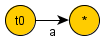
\includegraphics[scale=0.5]{2.png}

For a string $s =" aa"$ :

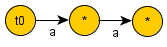
\includegraphics[scale=0.5]{3.png}

For a string $s =" ab"$ :

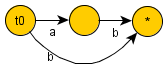
\includegraphics[scale=0.5]{4.png}

For a string $s =" aba"$ :

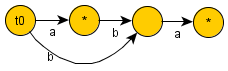
\includegraphics[scale=0.5]{5.png}

For a string $s =" abb"$ :

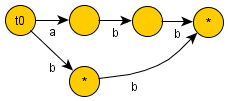
\includegraphics[scale=0.5]{6.png}

For a string $s =" abbb"$ :

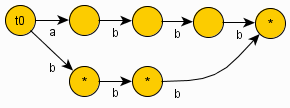
\includegraphics[scale=0.5]{7.png}

\subsection{ Algorithm for constructing the suffix automaton in linear time }

Before you go directly to the description of the algorithm construction, it is necessary to introduce some new concepts and demonstrate a simple, but very important for the understanding of suffix automaton of the lemma.

\subsubsection{ Position endings. Properties and relationship with the suffix automaton }

Consider any non-empty substring $t$ line $s$. Then called the \textbf{set of endings} $endpos (t)$ set of all positions in the line $s$ In which the end of the lines with $t$.

We will call two substrings $t_1$ and $t_2$$endpos$ Equivalent if their sets of endings are the same: $endpos (t_1) = endpos (t_2)$. Thus, all non-empty substrings $s$ can be divided into several \textbf{classes} according to their \textbf{equivalence} sets $endpos$.

It turns out that the suffix automaton \textbf{$endpos$} \textbf{-Equivalent substring match the same state.} In other words, the number of states in the suffix automaton is the number of classes $endpos$ -Equivalence among all substrings, plus one initial state. Each state of the machine suffix match one or more substrings, having the same value $endpos$.

\textbf{This statement we take for granted,} and we describe an algorithm for constructing suffix automaton on that assumption - as we shall see later, all the required properties of suffix automaton, except minimum will be achieved. (A minimal follows from Theorem Nerode - see References).

We also present some simple but important statements about values $endpos$.

\textbf{Lemma 1.} Two nonempty substring $u$ and $w$($length (u) \le length (w)$)Are $endpos$ -Equivalent if and only if the line $u$ in the string $s$ only as a suffix string $w$.

The proof is almost obvious. One way: if $u$ and $w$ have the same position endings entry, then $u$ is a suffix $w$ And it is present in $s$ only as a suffix $w$. Conversely, if $u$ is a suffix $w$ and is only as this suffix, their values $endpos$ equal by definition.

\textbf{Lemma 2.} Consider two nonempty substring $u$ and $w$($length (u) \le length (w)$ ). Then they set $endpos$ either disjoint or $endpos (w)$ is contained in $endpos (u)$, And it depends on whether the $u$ suffix $w$ or not:

$\begin{cases}
endpos(w)\subset endpos(u) & {\rm if}\, u\,{\rm suffix}\, w\\
endpos(u)\cap endpos(w)=\emptyset & {\rm otherwise}
\end{cases}$

Proof. Assume that the sets $endpos (u)$ and $endpos (w)$ have at least one common element. Then it means that the line $u$ and $w$ end at the same place, i.e., $u$ - Suffix $w$. But then every occurrence of the string $w$ contains at its end of the entry line $u$, Which means that its set $endpos (w)$ entirely embedded in many $endpos (u)$.

\textbf{Lemma 3.} Consider a class of $endpos$ Equivalence. Sort all the strings that are included in this class, in decreasing length. Then, the resulting sequence of each substring will be shorter than the previous one, and thus is a suffix of the previous one. In other words, \textbf{substrings belonging to the same equivalence class, in fact, is a suffix to each other, and make all sorts of different lengths in an interval} \textbf{$[X; y]$}.

Proof.

Fix a class $endpos$ Equivalence. If it contains only one row, then the correctness of the lemma is obvious. Now suppose that the number of rows is more than one.

According to Lemma 1, the two different $endpos$ -Equivalent lines are always like that one is a proper suffix of another. Consequently, in the same class $endpos$ -Equivalence can not be strings of the same length.

We denote $w$ length, and a $u$ - The shortest line in the equivalence class. According to Lemma 1, Line $u$ is a proper suffix of $w$. We now consider any suffix string $w$ with a length of the interval $[Length (u); length (w)]$ And show that it is contained in the same equivalence class. In fact, this suffix can be included in $s$ only as a suffix string $w$ (Because the shorter suffix $u$ enters only as a suffix string $w$ ). Therefore, according to Lemma 1, this suffix $endpos$ Row-equivalent $w$, As required.

\subsubsection{ Suffix links }

Consider a state machine $v \ne t_0$. As we now know as $v$ corresponds to a class of rows with the same values $endpos$ Moreover, if we denote $w$ longest of these lines, then the others will suffixes $w$.

We also know that the first few lines of suffixes $w$ (If we consider the suffixes in descending order of length) are in the same equivalence class, and all other suffixes (or at least the empty suffix) - in some other classes. We denote $t$ first such suffix - in it we spend suffix link.

In other words, the \textbf{suffix link} $link (v)$ leads to a condition which corresponds \textbf{naidlinneyshy suffix} string $w$, Which is in a different class $endpos$ Equivalence.

Here we assume that the initial state $t_0$ corresponds to a single equivalence class (containing only the empty string), and we believe $endpos (t_0) = [-1 \ldots length (s) -1]$.

\textbf{Lemma 4.} Suffix links form a \textbf{tree,} whose root is the initial state $t_0$.

Proof. Consider an arbitrary state $v \ne t_0$. Suffix link $link (v)$ leading from it to a state corresponding to the string strictly shorter length (this follows from the definition of suffix links and Lemma 3). Therefore, moving the suffix links, we will sooner or later come from the state $v$ to the initial state $t_0$, Which corresponds to an empty string.

\textbf{Lemma 5.} If we build on all available sets $endpos$ \textbf{tree} (on a "many-to-parent contains a subset of all of their children"), it will be the same as the structure of the tree suffix links.

Proof.

The fact that the sets $endpos$ You can build a tree, from Lemma 2 (that any two sets $endpos$ either disjoint or one is contained in the other).

Now consider an arbitrary state $v \ne t_0$ and the suffix link $link (v)$. From the definition of suffix links and from Lemma 2:

$endpos (v) \subset endpos (link (v)),$

which together with the previous lemma proves our assertion tree suffix links is essentially a timber is laid sets $endpos$.

\textbf{Here is an example} of the tree suffix links in the suffix automaton constructed for the line $" abcbc"$ :

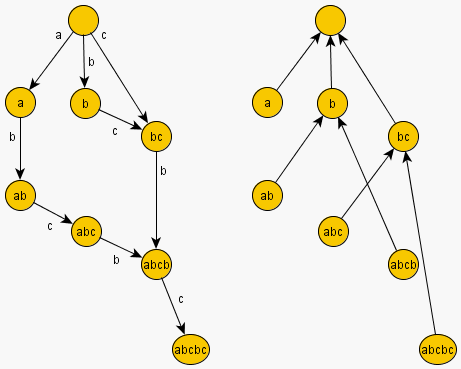
\includegraphics[scale=0.5]{8.png}

\subsubsection{ Summary }

Before proceeding to the algorithm itself, systematize knowledge accumulated over, and introduce a couple of auxiliary symbols.

Many substrings $s$ can be divided into equivalence classes according to their end of the sets $endpos$.
Suffix automaton consists of an initial state $t_0$, As well as one of each class $endpos$ Equivalence.
Each of $v$ corresponds to one or more rows. We denote $longest (v)$ longest of these lines through $len (v)$ its length. We denote $shortest (v)$ shortest of these lines, and its length by $minlen (v)$.
Then all the rows corresponding to this condition are various suffixes line $longest (v)$ and have all sorts of lengths in the interval $[Minlen (v); len (v)]$.

For each state, $v \ne t_0$ defined suffix link leading to a state that corresponds to the suffix string $longest (v)$ length $minlen (v) -1$. Suffix links form a tree rooted at the $t_0$, And this tree is actually a tree inclusion relations between sets $endpos$.
Thus, the $minlen (v)$ for $v \ne t_0$ expressed by the suffix links $link (v)$ as:
$minlen (v) = len (link (v)) + 1.$

If we start from an arbitrary state $v_0$ and will go to the suffix links, then sooner or later we get to the initial state $t_0$. In this case, we get a sequence of disjoint segments $[Minlen (v_i); len (v_i)]$ Which will merge one solid piece.
\subsubsection{ Algorithm for constructing the suffix automaton in linear time }

Proceed to the description of the algorithm itself. The algorithm is \textbf{online,} that is, will add one character string $s$ By rearranging accordingly the current machine.

To achieve linear memory consumption, in each state, we will only be stored value $len$, $link$ and a list of transitions from this state. Tags terminal conditions, we will not support (we show you how to place the labels after the construction of suffix automaton, if there is a need for them.)

\textbf{Initially the} machine consists of a single state $t_0$ We agree to assume zero state (other states will get a room $1, 2, \ldots$ ). Assign this state $len = 0$ And value $link$ assign a convenience $-1$ (A reference to a fictional, non-existent state).

Accordingly, the whole challenge now is to ensure that the implement process \textbf{of adding one character} $c$ at the end of the current line. We describe this process:

Let $last$ - A state that corresponds to the entire current line to add the character $c$. (Initially $last = 0$ And after the addition of each character, we will change the value of $last$.)
Create a new state $cur$ By placing him $len (cur) = len (last) + 1$. Value $link (cur)$ still considered uncertain.
We make such a cycle: initially we are able to $last$ And if he does not go out in the letter $c$, Then add the transition to the letter $c$ in state $cur$ And then go on suffix link to check again - if there is no transition, we add. If at any time it happens that such a transition is already there, then stop - and let $p$ number of the state in which it happened.
If you have never happened, that the passage in the letter; $c$ I already had, and we did come to a fictitious state $-1$ (In which we have come to the suffix link from the initial state $t_0$ ), We can simply set $link (cur) = 0$ and exit.
Suppose now that we stopped for some state $p$, From which there was a shift in the letter; $c$. We denote $q$ the state, which is available this transition.
Now we have two cases, depending on whether $len (p) + 1 = len (q)$ or not.
If $len (p) + 1 = len (q)$, We can simply set $link (cur) = q$ and exit.
Otherwise, everything is more complicated. Requires a \textbf{"cloning" of} the state $q$ : To create a new state $clone$ By copying all the data to it from the top $q$ (Suffix link transitions), except for the value $len$ : It is necessary to assign $len (clone) = len (p) + 1$.
After cloning, we spend suffix link from $cur$ in this state $clone$ Also redirect the suffix link from $q$ in $clone$.

Finally, the last thing we need to do - is to go on the state $p$ suffix on the links, and for each of the next state to check: if there was a transition in the letter $c$ in state $q$ Then forward it to the state $clone$ (And if not, then stop).

In any case, whatever over this procedure, we are at the end of the value being updated $last$, To be the $cur$.
If we also need to know which vertices are \textbf{terminal,} and what - no, we can find all terminal nodes after the construction of suffix automaton for the whole line. For this, consider the state corresponding to the whole line (which, obviously, we have stored in the variable $last$ ), And we will walk in his suffix links until we reach the initial state, and mark each covered condition as terminal. It is easy to understand that by doing so we mark the states corresponding to all suffix of $s$ That we required.

In the next section, we will look at each step of the algorithm and prove its \textbf{correctness.}

Here we only note that the algorithm shows that the addition of one character leads to the addition of one or two states in the machine. Thus, the \textbf{linearity of the number of states} is obvious.

The linearity of the number of transitions, and generally linear time algorithm less clear, and they will be proved below, after the proof of the correctness of the algorithm.

\subsubsection{ Proof of the correctness of the algorithm }

We say that the transition $(P, q)$ \textbf{solid,} if $len (p) + 1 = len (q)$. In the opposite case, i.e., when $len (p) + 1 <len (q)$, The transition is called \textbf{discontinuous.}
As can be seen from the description of the algorithm, solid and non-solid transitions lead to different branches of the algorithm. Solid transitions are so called because, having appeared for the first time, they will never be changed. In contrast, non-continuous transitions may change if you add new letters to the line (can change the end of the arc transition).

To avoid ambiguities, below the $s$ we mean the row for which the machine was built Suffix to add the current symbol $c$.
The algorithm starts with the fact that we are creating a new state $cur$ That will match the entire string $s + c$. Understand why we have to create a new state - as together with the addition of a new character, a new equivalence class - a class of lines ending in added symbol $c$.
After creating a new state of the algorithm is passed by the suffix links from the state corresponding to the entire line $s$, And trying to add a transition on the symbol $c$ in state $cur$. Thus, we attribute to each suffix string $s$ symbol $c$. But add new transitions, we can only be, if they do not conflict with existing ones, so as soon as we meet an existing transition from the symbol $c$ We must stop immediately.
The simplest case - if we did come to a fictitious state $-1$ Adding all the new characters move along $c$. This means that the character $c$ in a row $s$ before met. We have successfully added all the transitions, you just have to put suffix link status $cur$ - Obviously it must be equal $0$ Because of $cur$ in this case, the string matches all suffixes $s + c$.
The second case - when we came across an existing transition $(P, q)$. This means that we have tried to add a line to the machine $x + c$ (Where $x$ - Some suffix string $s$ Having a length $len (p)$ ), And this line \textbf{has been previously added} to the machine (i.e., line $x + c$ already included as a substring in a string $s$ ). Since we assume that the automaton for the string $s$ built correctly, the new transitions, we do not have more to add.
However, there is a difficulty with where to keep suffix link from the state $cur$. We need to spend suffix link to a condition in which the length of the string will be exactly this same $x + c$ i.e. $len$ for this condition should be equal $len (p) + 1$. However, such a state could not exist: in this case we need to produce a \textbf{"splitting" of the} state.

So, one of the possible scenarios, the transition $(P, q)$ was continuous, i.e. $len (q) = len (p) + 1$. In this case simple, no splitting of the produce is not necessary, and we just spend suffix link from the state $cur$ in state $q$.
Another more complicated option - when the discontinuous transition, i.e. $len (q)> len (p) + 1$. This means that the state $q$ corresponds not only necessary to us substring $w + c$ length $len (p) + 1$ But also a substring longer. We have no choice but to make a \textbf{"split"} status $q$ Smash the segment lines corresponding to her two subsegments, so the first will end up just $len (p) + 1$.
How to make this split? We \textbf{"clone"} state $q$ By making a copy of it $clone$ with parameter $len (clone) = len (p) + 1$. We copy in $clone$ of $q$ all the transitions, because we do not want in any way to change the path, pass through $q$. Suffix link from $clone$ we are there, reached by a link from the old suffix $q$ And the reference of $q$ send to $clone$.

After cloning, we spend suffix link from $cur$ in $clone$ - Something for which we cloned.

Final step - redirect some members of the $q$ transitions, forwarding them to the $clone$. What exactly must redirect incoming transitions? Just redirect the only transitions corresponding to all the suffix of $w + c$ i.e. we should continue to move in the suffix links, starting from the top $p$ And for as long as we get to a fictitious state $-1$ or do not go to the state, which is the transition from a state other than $q$.

\subsubsection{ Proof of linear operations }

First of all, just to mention, that we believe the alphabet size \textbf{constant.} If it is not, then talk about the linear running time will not work: the list of transitions from one node to be stored in the form of a B-tree allows fast searching by key, and the key is added. Therefore, if we denote $k$ size of the alphabet, then the asymptotic behavior of the algorithm will $O (n \log k)$ at $O (n)$ memory. However, if the alphabet is small, you can, sacrificing memory, avoid balanced lists, and keep the transitions at each node in an array of length $k$ (For a quick search on the key) and a dynamic list (for fast traversal of all available keys). Thus we reach $O (n)$ time of the algorithm, but at the cost $O (n k)$ memory consumption.

Thus, we assume a constant size of the alphabet, i.e. each search move for the symbol, add a transition, searching for the next move - all of these operations, we believe working for $O (1)$.

If we look at all parts of the algorithm, it has three seats, the linear asymptotics is not obvious:

First place - is the doorway to the state of the suffix links $last$ with the addition of ribs on the symbol $c$.
Second place - up state transitions during the cloning $q$ to a new state $clone$.
Third place - redirect transitions leading to $q$ On $clone$.
We use the well-known fact that the size of suffix automaton (both in number of states, and the number of hops) \textbf{is linear.} (The proof is linear in the number of states is the algorithm, and the proof is linear in the number of transitions given below, after the implementation of the algorithm.).

Then the obvious linear total asymptotics of the \textbf{first and second place:} for each operation is added to the machine one new transition.

It remains to estimate the total asymptotics \textbf{in third place} - the one where we redirect the transitions leading to $q$ On $clone$. Denote $v = longest (p)$. This suffix string $s$ And with each iteration of its length decreases - and, therefore, the position of $v$ as suffix string $s$ increases monotonically with each iteration. In this case, if before the first iteration of the loop corresponding row $v$ was at a depth of $k$($k \ge 2$)From $last$ (If you count the number of depth suffix links that you have to pass), after the last iteration of the line $v + c$ will $2$ St suffix referring to the path of $cur$ (Which becomes the new value $last$ ).

Thus, each iteration of this cycle leads to the fact that the position of the string $longest (link (link (last))$ as suffix entire current line will be monotonically increasing. Consequently, only this cycle could not work more $n$ iterations, \textbf{as required.}

(It is worth noting that similar arguments can be used to prove the linearity of the first place, instead of referring to the proof of the linearity of the number of states.)

\subsection{ Implementation of the algorithm }

First we describe the data structure that will hold all the information about a particular passage($len$, $link$, The list of transitions). If necessary, you can add a flag here is terminal, as well as other required information. The jump list we maintain in the form of a standard container $map$, Which allows for a total of $O (n)$ Memory and $O (n \log k)$ time to process the entire string.

\begin{verbatim}
struct state {
    int len, link ;
    map < char, int > next ;
} ; 
\end{verbatim}
Suffix machine itself will be stored in an array of these structures $state$. As is proved in the next section, if $MAXN$ - Is the maximum possible length of a line in the program, it is enough to have a memory for $2 \cdot MAXN - 1$ states. We also keep a variable $last$ - The state corresponding to the entire line at the moment.

\begin{verbatim}
const int MAXLEN = 100000 ;
state st[MAXLEN * 2];
int sz, last ; 
\end{verbatim}
We present a function that initializes Suffix Machine (creating machine with a single initial state):

\begin{verbatim}
void sa_init() {
    sz = last = 0 ;
    st[0].len = 0 ;
    st[0].link = - 1 ;
    ++ sz ;
    /*
    // This is needed only if the machine is constructed many times for different lines:
    for (int i=0; i<MAXLEN*2; ++i)
        st[i].next.clear();
    */
} 
\end{verbatim}
Finally, we present the implementation of the basic functions - which adds another character to the end of the current line, rearranging accordingly machine:

\begin{verbatim}
void sa_extend(char c){
    int cur = sz ++ ;
    st[cur].len = st[last].len + 1 ;
    int p ;
    for(p = last ; p ! = - 1 && ! st[p].next. count(c); p = st[p].link )
        st[p].next[c]= cur ;
    if(p == - 1 )
        st[cur].link = 0 ;
    else {
        int q = st[p].next[c];
        if(st[p].len + 1 == st[q].len )
            st[cur].link = q ;
        else {
            int clone = sz ++ ;
            st[clone].len = st[p].len + 1 ;
            st[clone].next = st[q].next ;
            st[clone].link = st[q].link ;
            for(; p ! = - 1 && st[p].next[c]== q ; p = st[p].link )
                st[p].next[c]= clone ;
            st[q].link = st[cur].link = clone ;
        }
    }
    last = cur ;
} 
\end{verbatim}
As mentioned above, if you sacrifice memory (up to $O (n k)$ Where $k$ - The size of the alphabet), you can reach build time machine $O (n)$ even for any $k$ - But you have to keep in each state array size $k$ (To quickly find the transition to the desired letter), and the list of transitions (for quick bypass or copy all transitions).

\subsection{ Additional properties of suffix automaton }

\subsubsection{ The number of states }

The number of states in the suffix automaton constructed for the line $s$ length $n$ Does \textbf{not exceed} \textbf{$2n-1$} (For $n \ge 3$ ).

This is proved by the above algorithm (as originally machine consists of one initial state, the first and second steps added in exactly the same state, and in each of the other $n-2$ steps could add two vertices from the splitting of state).

However, this estimate \textbf{is easy to show, and without the knowledge of the algorithm.} Let us remember that the number of states is equal to the number of different sets of values $endpos$. In addition, these sets $endpos$ form a tree on a "top of the parent contains a subset of all the children." Consider a tree, and a little transform it: as long as there is an internal node with one son, it means that $endpos$ this son does not contain at least one number from $endpos$ parent, then create a virtual node with $endpos$ Equal to that number, and weight gain of the son to the parent. As a result, we obtain a tree in which each internal vertex has degree greater than one, and the number of leaves is at most $n$. Consequently, only such a tree no more $2n-1$ top.

Thus we have shown that assessment independently, without knowledge of the algorithm.

It is interesting to note that this estimate is sharp, i.e. there is a \textbf{test in which it is achieved.} This test is as follows:

$" abbbb \ldots " $

When processing the string at each iteration, starting with the third, will be splitting of the state, and, thus, will be achieved score $2n-1$.

\subsubsection{ The number of transitions }

The number of transitions in the suffix automaton constructed for the line $s$ length $n$ Does \textbf{not exceed} \textbf{$3n-4$} (For $n \ge 3$ ).

\textbf{Prove} it.

We estimate the number of continuous transitions. Consider a spanning tree of the longest path in the machine, starting in state $t_0$. This frame will consist of the solid edges, and, consequently, the number is one less than the number of states, i.e., does not exceed $2n-2$.

We now estimate the number of non-continuous transitions. Let us consider each non-solid transition, and let the current transition - a transition $(P, q)$ the symbol $c$. Put it in the appropriate line $u + c + w$, Where row $u$ corresponding long way from the initial state to $p$ And $w$ - The length of the path $q$ in any terminal state. On the one hand, all these lines $u + c + w$ for all non-continuous transitions are different (because the strings $u$ and $w$ formed only by solid transitions). On the other hand, each of these lines $u + c + w$ By definition of the terminal condition, the entire line will be suffixed $s$. As a non-empty suffix string $s$ only $n$ pieces, and also the entire line $s$ of these lines $u + c + w$ could not be contained (as the whole line $s$ corresponds to the path of $n$ solid edges), then the total number of non-continuous transitions does not exceed $n-1$.

Combining these two estimates, we obtain $3n-3$. However, remembering that the maximum number of states can only be achieved on the test form $" abbbb \ldots "$, And its assessment $3n-3$ clearly not achieved, we get the final estimate $3n-4$, As required.

Interestingly, there is also a \textbf{test on which this estimate is achieved by:}

$" abbb \ldots bbbc" $

\subsubsection{ Relation with suffix tree. Construction of suffix tree with suffix automaton and vice versa }

We prove two theorems that establish the mutual relationship between the suffix automaton and suffix tree.

Outset that we believe that the input line is that each has its own suffix in the suffix tree top (as for arbitrary strings, generally speaking, is not true: for example, the string $" aaa \ldots"$ ). This is usually achieved through the attribution to the end of line for some special characters (usually denoted by a dollar sign).

For convenience we introduce the notation: $\overline {s}$ - A string $s$ Written in reverse order, $DAWG (s)$ - Suffix this machine, built for the line $s$, $ST (s)$ - Is a suffix tree line $s$.

We introduce the notion of \textbf{expanding links:} fix suffix tree top $v$ and symbol $c$, Then expands link $ext [c, v]$ leads to the top of the tree at line $c + v$ (If this path $c + v$ ends in the middle of the edge, then hold a reference to the lower end of the edge), and if such a path $c + v$ does not exist in the tree, then extending the link is not defined. In a sense, the opposite of expanding links suffix links.

\textbf{Theorem 1.} Tree formed by the suffix links $DAWG (s)$, Is the suffix tree $ST (\overline {s})$.

\textbf{Theorem 2.} $DAWG (s)$ - A graph of links extending suffix tree $ST (\overline {s})$. In addition, the solid edges in $DAWG (s)$ - Is inverted suffix links $ST (\overline {s})$.

These two results enable one to one of the structures (the suffix tree or the suffix automaton) to build another in time $O (n)$ - These two simple algorithms will be reviewed by us below in Theorems 3 and 4.

For illustrative purposes, we present the machine with its Suffix tree suffix links and the corresponding suffix tree for the inverted row. For example, take a string $s =" abcbc"$.

$DAWG (" abcbc")$ and the suffix tree of links (for clarity, we will sign it, each state $longest$ -Line):

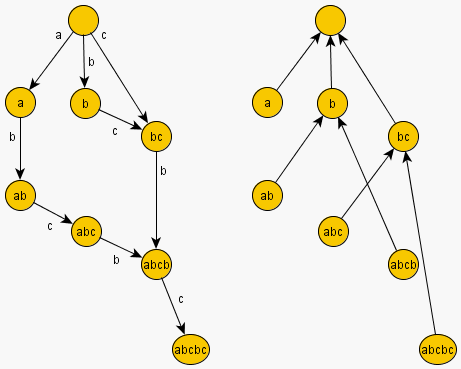
\includegraphics[scale=0.5]{9.png}

$ST (" cbcba")$ :

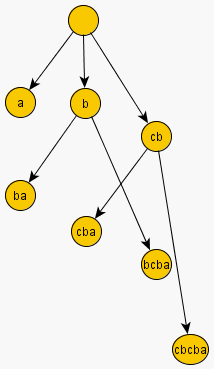
\includegraphics[scale=0.5]{10.png}

\textbf{Lemma.} The following three statements are equivalent for any two substrings $u$ and $w$ :

$endpos (u) = endpos (w)$ in a row $s$

$firstpos (\overline {u}) = firstpos (\overline {w})$ in a row $\overline {s}$

$\overline {u}$ and $\overline {w}$ lie on the same path from the root to the suffix tree $ST (\overline {s})$.
Its proof is quite obvious: if the start of the two occurrences of the same lines, one line is a prefix of the other, and, therefore, one line is in the suffix tree on a different row.

\textbf{Theorem 1.}

Status suffix automaton correspond to the vertices of suffix tree.

Consider a suffix link $y = link (x)$. By the definition of suffix links $longest (y)$ is a suffix $longest (x)$, And among all of these $y$ choose the one with the $len (y)$ maximum.

In terms of the inverted row $\overline {s}$ this means that the suffix link $link [x]$ leads to a longer prefix string corresponding to the state $x$ To this prefix corresponds separate state $y$. In other words, the suffix link $link [x]$ leads to the top of the ancestor $x$ in the suffix tree, as required.

\textbf{Theorem 2.}

Status suffix automaton correspond to the vertices of suffix tree.

Consider any transition $(X, y, c)$ in suffix automaton $DAWG (s)$. The presence of this transition means that $y$ - It is a condition, the equivalence class that contains the substring $longest (x) + c$. In the inverted row $\overline {s}$ This means that $y$ it is a condition which corresponds to the substring $firstpos$ of which (in the text $\overline {s}$)Coincides with $firstpos$ by substring $c + \overline {longest (x)}$.

It just means that:

$\overline{longest(y)}=ext[c,\overline{longest(x)}]$

The first part of the theorem, it remains to prove the second part: that all solid transitions in the machine correspond to the links in the suffix tree. Continuous transition is different from the non-exhaustive because $length (y) = length (x) + 1$ i.e. After assigning a character $c$ we are in a state with a string of maximum equivalence class of this state. This means that when calculating the appropriate spreading links $ext [c, \overline {longest (x)}]$ We immediately hit the top of the tree, rather than going down to the nearest node of a tree. Thus, assigning a single character in the beginning, we got to the top of another tree - so if this is the inverted suffix link in the tree.

The theorem is proved.

\textbf{Theorem 3.} With automatic Suffix $DAWG (s)$ Can be a time $O (n)$ build a suffix tree $ST (\overline {s})$.

\textbf{Theorem 4.} With suffix tree $ST (\overline {s})$ Can be a time $O (n)$ Suffix build machine $DAWG (s)$.

\textbf{Proof of Theorem 3.}

Suffix tree $ST (\overline {s})$ will contain the same number of vertices in many states $DAWG (s)$, And the top of the tree, resulting from the state of $v$ automaton corresponds to a string of length $len (v)$.

According to Theorem 1, the edges of the tree are formed as inverted suffix links and arc labels can be found, based on the difference $len$ states, and further knowing each state machine of any one element of his set $endpos$ (This is one element of $endpos$ You can support the construction of the machine).

Suffix link in the tree, we can construct, by Theorem 2: it is enough to see all the solid transitions in the machine, and for each such transition $(X, y)$ Add a link $link (y) = x$.

Thus, over time, $O (n)$ we can build a suffix tree with a suffix link in it.

(If we consider the size of $k$ alphabet is not constant, then all it will take time to rebuild $O (n \log k)$.)

\textbf{Theorem 4.}

Suffix Machine $DAWG (s)$ will contain the same number of states as vertices $ST (\overline {s})$. Each state $v$ His long string $longest (v)$ will correspond to the inverted path from the root of the tree to the top $v$.

By Theorem 2, to build all the transitions in the suffix automaton, we need to find all the links expand $ext [c, v]$.

First, note that some of these links extend obtained directly from the links in the suffix tree. In fact, if for any vertex $x$ we consider its suffix link $y = link (x)$ It means that it is necessary to hold the expanding link from $y$ in $x$ first-character string corresponding to the vertex $x$.

However, since we do not find an expanding links. Additionally it is necessary to walk on the suffix tree from the leaves to the root, and for each vertex $v$ View all of her sons, each son see all expanding links $ext [c, w]$, And copy the link to the top $v$ If this symbol $c$ link from the top $v$ has not yet been found:

$ext[c,v]=ext[c,w]\qquad{\rm if}\, ext[c,w]=nil$

This process worked during $O (n)$ If we consider the size of the alphabet constant.

Finally, it remains to construct the suffix links in the machine, but, according to Theorem 1, the suffix links obtained simply as the ribs of suffix tree $ST (\overline {s})$.

Thus, this algorithm in time $O (n)$ Suffix machine builds on the suffix tree for the inverted row.

(If we believe that the size of $k$ alphabet - as a variable, then the asymptotic behavior will increase to $O (n \log k)$.)

\subsection{ Usage in solving problems }

We'll see what can be done with the suffix automaton.

For simplicity, we assume the size of the alphabet $k$ constant, which will allow us to consider the asymptotic behavior of the construction of suffix automaton and pass on it constant.

\subsubsection{ Checking entry }

\textbf{Condition.} Given text $T$, The request is received in the form: given a string $P$, You want to check is whether or not the string $P$ in the text $T$ as a substring.

\textbf{Asymptotics.} Preprocessing $O (length (T))$ and $O (length (P))$ one request.

\textbf{Decision.} Construct an automaton on the text Suffix $T$ during $O (length (T))$.

As it is now responding to a single request. Let the current state - it is a variable $v$ It is initially equal to the initial state $t_0$. We will go for a character string $P$, As appropriate, making the transition from the current state $v$ a new state. If at any time it happened that the transition from the current state to the desired character was not - the response to "no." If we are unable to process the entire line $P$, The response to "yes."

It is clear that this will work for the time $O (length (P))$. Moreover, the algorithm is actually looking length of the longest prefix $P$ In the text - and if the input patterns are such that these distances are small, then the algorithm will run much faster without all the processing line entirely.

\subsubsection{ The number of different substrings }

\textbf{Condition.} Given a string $S$. Need to know the number of its different substrings.

\textbf{Asymptotics.} $O (length (S))$.

\textbf{Decision.} Suffix to construct an automatic line $S$.

In the suffix automaton any substring $S$ corresponds to a path in the machine. Since the duplicate rows in the machine can not be the answer to the problem - \textbf{how} many \textbf{different ways} in the machine, starting at the initial vertex $t_0$.

Given that Suffix automaton is an acyclic graph, the number of different ways it can be considered by the dynamic programming.

Namely, let $d [v]$ - The number of different ways, starting with the state $v$ (Including the path length of zero.) Then we have:

$d[v]=1+\sum_{w:
(v,w,c)\in{\rm DAWG}}d[w]$

i.e. $d [v]$ can be expressed as the sum of responses to all possible transitions from state $v$.

Answer to the problem is the value of $d [t_0] -1$ (A unit is taken away to ignore the empty substring).

\subsubsection{ The total length of different substrings }

\textbf{Condition.} Given a string $S$. Want to know the total length of all its different substrings.

\textbf{Asymptotics.} $O (length (S))$.

\textbf{Decision.} Solution of the same as above, only now we have to consider the dynamics of two values: the number of different substrings $d [v]$ and the total length $ans [v]$.

How to count $d [v]$, Described in the previous task, and the value $ans [v]$ can be calculated as follows:

$ans[v]=1+\sum_{w:
(v,w,c)\in{\rm DAWG}}d[w]+ans[w]$

i.e. we take the response for each vertex $w$, And add to it $d [w]$ Thus, as it were attributing to the beginning of each line of one character.

\subsubsection{ Lexicographically k-th substring }

\textbf{Condition.} Given a string $S$. GET requests - the number of $K_i$ And the need to find $K_i$ Th in the sort order substring $S$.

\textbf{Asymptotics.} $O (length (ans) \cdot Alphabet)$ one request (where $ans$ - A response to this request, $Alphabet$ - The size of the alphabet).

\textbf{Decision.} The solution to this problem is based on the same idea as the previous two problems. Lexicographically $k$ Th substring - is lexicographic $k$ First way to suffix automaton. Therefore, considering for each state of the ways out of it, we will be able to easily search $k$ First way, moving from the root machine.

\subsubsection{ The smallest cyclic shift }

\textbf{Condition.} Given a string $S$. Required to find the lexicographically smallest of its cyclic shift.

\textbf{Asymptotics.} $O (length (S))$.

\textbf{Decision.} Suffix to construct an automatic line $S + S$. Then this machine will contain a path all cyclic shifts of the string $S$.

Consequently, the problem reduces to that found in the machine lexicographically minimum path length $length (S)$ That is done in a trivial way: we start in the initial state, and each time act greedily, moving the transition with minimal character.

\subsubsection{ Number of occurrences }

\textbf{Condition.} Given text $T$, The request is received in the form: given a string $P$, Want to know how many times the line $P$ included in the text $T$ as a substring (occurrences may overlap).

\textbf{Asymptotics.} Preprocessing $O (length (T))$ and $O (length (P))$ one request.

\textbf{Decision.} Construct an automaton on the text Suffix $T$.

Next we need to do this preprocessing: for each state $v$ machine to count the number $cnt [v]$ Equal to the size of the set $endpos (v)$. In fact, all the rows corresponding to the same state, are $T$ the same number of times as the number of items in the set $endpos$.

But clearly supports many $endpos$ for all states, we can not, so learn to read only their size $cnt$.

To do this, proceed as follows. For each state, if it was not obtained by cloning (and the initial state $t_0$ We also do not count), initially assign $cnt = 1$. Then we will go over all the states in order of their length $len$ and the current value of the port-forwarded $cnt [v]$ suffix on this link:

$cnt [link (v)] + = cnt [v].$

States that in the end we have to calculate the correct value of each state $cnt$.

Why is this true? All states obtained by cloning is not, exactly $length (S)$ And $i$ St of them came when we added the first $i$ characters. Consequently, each of these states, we associate this position, the processing of which it appeared. Therefore, initially, each such condition $cnt = 1$, And in all other states $cnt = 0$.

Then we perform for each $v$ this operation: $cnt [link (v)] + = cnt [v]$. The meaning of this is that if the row corresponding to the state $v$, Met $cnt [v]$ time, all its suffixes will meet the same.

Why thus we do not take into account the same position a few times? Because of the value of each state "forwarding an" only once, so it could well be that one state it is "icing" to some other state twice, in two different ways.

Thus, we have learned to take these values $cnt$ for all states of the automaton.

After that prompted trivial - just return $cnt [t]$ Where $t$ - The state corresponding to the model $P$.

\subsubsection{ The position of the first occurrence }

\textbf{Condition.} Given text $T$, The request is received in the form: given a string $P$, Want to know the position of the start of the first occurrence of the string $P$.

\textbf{Asymptotics.} Preprocessing $O (length (T))$ and $O (length (P))$ one request.

\textbf{Decision.} Construct an automaton on the text Suffix $T$.

To solve the problem, we also need to add a preprocessing to find positions $firstpos$ for all states of the automaton, i.e. for each state $v$ we want to find a position $firstpos [v]$ end of the first occurrence. In other words, we want to find in advance the minimum element of each of the sets $endpos (v)$ (Because obviously support all sets $endpos$ we can not).

\textbf{Maintain} this position $firstpos$ easiest to right during the build machine: when we create a new state $cur$ when the function $sa \_extend()$ Then expose him:

$firstpos (cur) = len (cur) - 1$

(If we are working in $0$ -Indexing).

In cloning the top $q$ in $clone$ we set:

$firstpos (clone) = firstpos (q),$

(As another option value, only one - it $firstpos (cur)$, Which is clearly more).

Thus, the answer to the inquiry - it's just $firstpos (t)-length (P) +1$ Where $t$ - The state corresponding to the model $P$.

\subsubsection{ The positions of all occurrences }

\textbf{Condition.} Given text $T$, The request is received in the form: given a string $P$ Is required to bring the positions of all its occurrences in a string $T$ (Occurrences can overlap).

\textbf{Asymptotics.} Preprocessing $O (length (T))$. Response to a request for $O (length (P) + answer (P))$ Where $answer (P)$ - The size of a response, i.e., We will solve the problem for the time order of the input and output.

\textbf{Decision.} Construct an automaton on the text Suffix $T$. Similarly to the previous problem, calculate the build process for each state of the machine position $firstpos$ end of the first occurrence.

Now suppose that the request - the line $P$. Find which state $t$ it corresponds.

It is clear that $firstpos (t)$ definitely should be part of the answer. What other positions have to find? We took into account the state of the machine containing the string $P$, But did not consider other conditions that correspond to these lines that $P$ is their suffix.

In other words, we need to find all the states of which \textbf{is achievable by the suffix links} state $t$.

Therefore, to solve the problem we need to keep for each state suffix list of links leading to it. Response to a request then will be how to make a \textbf{detour to the depth / width} of these inverted suffix links from state $t$.

This diversion will operate during $O (answer (P))$ Because we do not visit the same state twice (because of the state of each suffix link goes only one, so no two paths leading to the same state).

However, we must bear in mind that the two-state values $firstpos$ \textbf{may be the same:} if one state was obtained by cloning another. However, this does not affect the asymptotic behavior, as each non-cloned vertex can be a maximum of one clone.

Moreover, you can easily get rid of the output repeats the position if we do not add back $firstpos$ the states of the clone. In fact, in any state-clone leads suffix link from the initial state, which is a condition to clone. Thus, if we remember each state flag $is \_clon$ And will not add to the answer $firstpos$ of conditions for which $is \_clon = true$, We thus obtain all required $answer (P)$ positions without repeats.

We present an outline of implementation:

\begin{verbatim}
struct state {
   ...
    bool is_clon ;
    int first_pos ;
    vector < int > inv_link ;
} ;
 
 
... after the construction of the machine...
for(int v = 1 ; v < sz ; ++ v )
    st[st[v].link].inv_link. push_back(v);
...
 
 
// Response to the request - the withdrawal of all occurrences (possibly with repetitions)
void output_all_occurences(int v, int P_length){
    if(! st[v].is_clon )
        cout << st[v].first_pos - P_length + 1 << endl ;
    for(size_t i = 0 ; i < st[v].inv_link. size() ; ++ i )
        output_all_occurences(st[v].inv_link[i], P_length);
} 
\end{verbatim}
\subsubsection{ Find the shortest string not in the text }

\textbf{Condition.} Given a string $S$ And set to a specific alphabet. Required to find a string of minimal length that it is not found in $S$ as a substring.

\textbf{Asymptotics.} The decision is $O (length (S))$.

\textbf{Decision.} Dynamic programming will decide on a machine, built for the line $S$.

Let $d [v]$ - Is the answer to the top $v$ i.e. We have already gained a substring part, being able to $v$ And we want to find the smallest number of characters that must add, to go beyond the machine, finding a nonexistent transition.

Considered $d [v]$ very simple. If the $v$ no transition at least one character in the alphabet, $d [v] = 1$ : Can we attribute this character and go beyond the machine, thus obtaining a search string.

Otherwise, a single character do not work, so we must take a minimum of the answers to all possible characters:

$d[v]=1+\sum_{w:
(v,w,c)\in{\rm DAWG}}d[w]$

Answer to the problem will be equal $d [t_0]$, And the string can be recovered and restored, how the dynamics turned this minimum.

\subsubsection{ Naidlinneyshaya common substring of two strings }

\textbf{Condition.} Given two strings $S$ and $T$. Need to find their naidlinneyshuyu common substring, i.e. this line $X$ That it is a substring and $S$ And $T$.

\textbf{Asymptotics.} The decision is $O (length (S) + length (T))$.

\textbf{Decision.} Suffix to construct an automatic line $S$.

We will now go on line $T$ And for each prefix search naidlinneyshy Suffix prefixes in $S$. In other words, we have for each position in the string $T$ naidlinneyshuyu want to find common substring $S$ and $T$ Ending is in this position.

For this purpose, we maintain two variables: \textbf{the current state of} $v$ and \textbf{the current length} $l$. These two variables will describe the current corresponding parts: its length and the state that corresponds to it (without storage length can not be avoided, since one state can match multiple strings of different lengths).

Initially $p = t_0$, $l = 0$ i.e. coincidence empty.

Now let us consider the symbol $T [i]$ and we want to count an answer for him.

If the state of $v$ in the machine, there is a transition from the symbol $T [i]$, We simply accomplish this transition, and increase $l$ by one.
If the state of $v$ not have the required transition, then we should try to shorten the current matching portion, which should go on suffix link:
$v = link (v).$

The ongoing need to shorten the length, but leave the maximum possible. Obviously, it should be assigned to $l = len (v)$ Because after you pass by suffix link us to satisfy any substring of length corresponding to this state:

$l = len (v).$

If the new state would not go back to the desired character, then we again have to go through the link and reduce the suffix $l$, And so on, until we find the transition (then go to step 1) or we do not get to a fictitious state $-1$ (Which means that the symbol $T [i]$ does not occur in $S$ Therefore assign $v = l = 0$ and go to the next $i$ ).

Answer to the problem will be a maximum of values $l$ for the time of the crawl.

Asymptotics of this passage is $O (length (T))$ Because in one move, we can either increase by one $l$ Or to make multiple passes over the suffix link, each of which will severely reduce the value $l$. Therefore, the decrease could not be more $length (T)$, Which means that the linear asymptotic behavior.

Implementation:

\begin{verbatim}
string lcs(string s, string t){
    sa_init() ;
    for(int i = 0 ; i <(int)s. length() ; ++ i )
        sa_extend(s[i ]);
 
    int v = 0,  l = 0,
        best = 0,  bestpos = 0 ;
    for(int i = 0 ; i <(int)t. length() ; ++ i){
        while(v && ! st[v].next. count(t[i ])) {
            v = st[v].link ;
            l = st[v].length ;
        }
        if(st[v].next. count(t[i ])) {
            v = st[v].next[t[i]] ;
            ++ l ;
        }
        if(l > best )
            best = l,  bestpos = i ;
    }
    return t. substr(bestpos - best + 1, best);
} 
\end{verbatim}
\subsubsection{ Most common substring of multiple strings. }

\textbf{Condition.} Dana $K$ lines $S_i$. Need to find their naidlinneyshuyu common substring, i.e. this line $X$ That it is a substring of $S_i$.

\textbf{Asymptotics.} The decision is $O (\sum length (S_i) \cdot K)$.

\textbf{Decision.} Merge all lines $S_i$ in one line $T$ By assigning to each line $S_i$ your own delimiter $D_i$ (i.e., entering $K$ extra special. Character $D_i$ )

$T = S_1 ~ D_1 ~ S_2 ~ D_2 ~ \ldots ~ S_k D_k.$

We construct the string $T$ Suffix automaton.

Now we need to find a line in the machine, which is contained in all rows $S_i$, And this will help us spices. characters. Note that if a substring occurs in some row $S_j$, The suffix automaton of the substring exists a path containing a character $D_j$ And contains no other characters $D_1, \ldots, D_ {j-1}, D_ {j +1}, \ldots, D_k$.

Thus, we need to calculate the reachability: for each state of the machine and each character $D_i$ there is a path that contains a separator $D_i$ And containing no other separators. This is easily done in a crawl depth / width or lazy dynamics. After that, the answer to the problem is the string $longest (v)$ for state $v$ Of which were found in all the way characters.

\subsection{ Tasks in the online judges }

Tasks that can be solved with suffix automaton:

SPOJ 7258 SUBLEX \textbf{"Lexicographical Substring Search"} [Difficulty: Medium]

\subsection{ Literature }

We start with a list of the first studies related to suffix automata

A. Blumer, J. Blumer, A. Ehrenfeucht, D. Haussler, R. \textbf{McConnell. Linear Size Finite Automata for the Set of All Subwords of a Word.} \textbf{An Outline of Results} [1983]
A. Blumer, J. Blumer, A. Ehrenfeucht, D. Haussler. \textbf{The Smallest Automaton Recognizing the Subwords of a Text} [1984]
Maxime Crochemore. \textbf{Optimal Factor Transducers} [1985]
Maxime Crochemore. \textbf{Transducers and Repetitions} [1986]
A. Nerode. \textbf{Linear automaton transformations} [1958]
In addition, more contemporary sources, this topic is touched upon in many books on string algorithms:

Maxime Crochemore, Wowjcieh Rytter. \textbf{Jewels of Stringology} [2002]
Bill Smyth. \textbf{Computing Patterns in Strings} [2003]
Bill Smith. \textbf{Methods and calculation algorithms on strings} [2006]

\section{ Finding all palindromes }
\subsection{ Statement of the problem }

Given a string $s$ length $n$. You want to find all the pairs $(I, j)$ Where $i <j$ That substring $s [i \ldots j]$ is a palindrome (i.e. reads the same from left to right and right to left).

\subsubsection{ Clarification of statement }

Clearly, in the worst case, such substrings, palindromes can be $O (n ^ 2)$, And at first glance it seems that the algorithm with linear asymptotics can not exist.

However, information about the found palindromes can return more \textbf{compact:} for each position $i = 0 \ldots n-1$ we find the values $d_1 [i]$ and $d_2 [i]$ Denoting the number of palindromes, respectively odd and even length with center position $i$.

For example, in the string $s = abababc$ There are three odd length palindrome with center symbol $s [3] = b$ i.e. value $d_1 [3] = 3$ :

$a\overbrace{ba\underbrace{b}_{s_{3}}ab}^{d_{1}[3]=3}c$

In line $s = cbaabd$ There are two palindrome of even length with the center in the symbol $s [3] = a$ i.e. value $d_2 [3] = 2$ :

$c\overbrace{ba\underbrace{a}_{s_{3}}b}^{d_{2}[3]=2}d$

i.e. idea - that if there is a length podpalindrom $l$ centered at some position $i$ That is, as long podpalindromy $l-2$, $l-4$, Etc. with centers $i$. Therefore, two such arrays $d_1 [i]$ and $d_2 [i]$ enough to store all podpalindromah this line.

Rather unexpected fact is that there is a fairly simple algorithm that calculates these "arrays palindromic" $d_1 []$ and $d_2 []$ in linear time. This algorithm is described in this article.

\subsection{ Decision }

Generally speaking, this problem has several known solutions: using a hashing technique can be solved $O (n \log n)$ And using suffix trees and fast algorithm LCA this problem can be solved $O (n)$.

However, described in this paper, the method is much simpler and has fewer hidden constants in the asymptotic time and memory. This algorithm was discovered \textbf{by Glenn Manakerom (Glenn Manacher)} in 1975

\subsubsection{ Trivial algorithm }

To avoid ambiguity in the further description of the conditions, what is a "trivial algorithm."

This algorithm, which to find an answer at the position $i$ repeatedly tries to increase the response by one, each time comparing the pair of corresponding symbols.

This algorithm is too slow, the whole answer he may deem just in time $O (n ^ 2)$.

Are representative of its implementation:

\begin{verbatim}
vector < int > d1(n ),  d2(n);
for(int i = 0 ; i < n ; ++ i){
    d1[i]= 1 ;
    while(i - d1[i]>= 0 && i + d1[i]< n && s[i - d1[i]] == s[i + d1[i]] )
        ++ d1[i];
 
    d2[i]= 0 ;
    while(i - d2[i]- 1 >= 0 && i + d2[i]< n && s[i - d2[i]- 1]== s[i + d2[i]] )
        ++ d2[i];
} 
\end{verbatim}
\subsubsection{ Algorithm Manakera }

Learn how to find all podpalindromy odd length, i.e. compute array $d_1 []$, Solution for palindromes of even length (i.e. finding array $d_2 []$)A slight modification of this.

For a quick calculation will support \textbf{border} \textbf{$(L, r)$} rightmost of the detected podpalindroma (i.e. with the highest podpalindroma $r$ ). Initially, you can put $l = 0, r = -1$.

Thus, suppose we want to calculate the value of $d_1 [i]$ for the next $i$, All previous values $d_1 []$ already counted.

If $i$ is not within the current podpalindroma, i.e. $i> r$, Please do the trivial algorithm.
i.e. will consistently increase the value $d_1 [i]$ And check every time - though whether the current substring $[I-d_1 [i]; i + d_1 [i]]$ is a palindrome. When we find the first difference, or when we get to the border line $s$ - Stop: we finally calculate the value $d_1 [i]$. After that, we have to remember to update the values $(L, r)$.

Consider now the case where $i \le r$.
Try to extract some information from the already calculated values $d_1 []$. Namely, to reflect the position $i$ inside podpalindroma $(L, r)$ i.e. Get the position $j = l + (r - i)$, And consider the value of $d_1 [j]$. Since $j$ - A position symmetrical position $i$, \textbf{Almost always} we can simply set $d_1 [i] = d_1 [j]$. An illustration of this reflection (palindrome around $j$ actually "copied" in palindrome around $i$ )

$\ldots\overbrace{s_{l}\ldots\underbrace{s_{j-d_{1}[j]+1}\ldots s_{j}\ldots s_{j+d_{1}[j]-1}}_{{\rm palindrome}}\ldots\underbrace{s_{i-d_{1}[j]+1}\ldots s_{i}\ldots s_{i+d_{1}[j]-1}}_{{\rm palindrome}}\ldots s_{r}\ldots}^{{\rm palindrome}}$

However, there are \textbf{subtleties} that must be processed correctly: when "internal palindrome" reaches the boundary of the outer or climbs over it, i.e., $j-d_1 [j] +1 \le l$ (Or, equivalently, $i + d_1 [j] -1 \ge r$ ). As for the external borders of the palindrome is no symmetry is not guaranteed, then just assign $d_1 [i] = d_1 [j]$ is already correctly: we have enough data to say that the position of $i$ podpalindrom has the same length.

In fact, to properly handle these situations, we must "cut" podpalindroma length, i.e. assign $d_1 [i] = r - i$. After that you should let a trivial algorithm that will try to increase the value $d_1 [i]$ As this is possible.

An illustration of this case (the one with a palindrome with center $j$ shows already "clipped" to such a length that it is placed right next to the outside palindrome)

$\ldots\overbrace{\underbrace{s_{l}\ldots s_{j}\ldots s_{j+(j-l)}}_{{\rm palindrome}}\ldots\underbrace{s_{i-(r-i)}\ldots s_{i}\ldots s_{r}}_{{\rm palindrome}}}^{{\rm palindrome}}\underbrace{\ldots\ldots\ldots\ldots\ldots}_{{\rm try\ }{\rm moving\ }{\rm here}}$

(This figure shows that while the palindrome centered at position $j$ could have been longer, beyond the scope of the external palindrome - but the position $i$ we can only use that part of it which is all the way into the outer palindrome. But the response to the position of $i$ may be more than this part, so then we have to run a trivial search, which will try to push it off the external palindrome, i.e. in the region "try moving here".)

At the end of the description of the algorithm just happened to recall that we must not forget to update the values $(L, r)$ after calculating the next value $d_1 [i]$.

Also be noted that the above reasoning, we have described for the calculation of an array of odd palindromes $d_1 []$, For an array of even palindromes $d_2 []$ All the arguments are similar.

\subsubsection{ Asymptotic estimation algorithm Manakera }

At first glance it is not obvious that this algorithm has a linear asymptotic form to calculate the answer to a particular position in it often runs a trivial search algorithm palindromes.

However, a more careful analysis shows that the algorithm is still linear. (It should refer to the well-known algorithm of Z-string functions, which internally resembles the algorithm, and also works in linear time.)

In fact, it is easy to trace the algorithm that each iteration produced trivial search, leads to an increase of one border $r$. This decrease in $r$ in the course of the algorithm can not occur. Consequently, the trivial algorithm will make a total of only $O (n)$ action.

Given that, except for trivial searches, all other parts of the algorithm Manakera obviously work in linear time, we get the final asymptotics $O (n)$.

\subsubsection{ Implementation of the algorithm Manakera }

For the case podpalindromov odd length, i.e. to compute the array $d_1 []$, We obtain the following code:

\begin{verbatim}
vector < int > d1(n);
int l = 0, r = - 1 ;
for(int i = 0 ; i < n ; ++ i){
    int k =(i > r ? 0 : min(d1[l + r - i], r - i)) + 1 ;
    while(i + k < n && i - k >= 0 && s[i + k]== s[i - k ]) ++ k ;
    d1[i]= k -- ;
    if(i + k > r )
        l = i - k,  r = i + k ;
} 
\end{verbatim}
Podpalindromov for even length, i.e. to compute the array $d_2 []$ Only slightly changed arithmetic expressions:

\begin{verbatim}
vector < int > d2(n);
l = 0, r = - 1 ;
for(int i = 0 ; i < n ; ++ i){
    int k =(i > r ? 0 : min(d2[l + r - i + 1], r - i + 1)) + 1 ;
    while(i + k - 1 < n && i - k >= 0 && s[i + k - 1]== s[i - k ]) ++ k ;
    d2[i]= -- k ;
    if(i + k - 1 > r )
        l = i - k,  r = i + k - 1 ;
} 
\end{verbatim}
\subsection{ Tasks in the online judges }

List of tasks that can be taken with the use of this algorithm:

UVA 11475 \textbf{"Extend to Palindrome"} [Difficulty: Easy]
\section{ Lyndon decomposition. Smallest cyclic shift }
\subsection{ The concept of decomposition Lyndon }

We define the concept \textbf{of decomposition Lyndon} (Lyndon decomposition).

Line is called \textbf{simple} if it is strictly \textbf{smaller than} any of its own \textbf{suffix.} Examples of simple lines: $a$, $b$, $ab$, $aab$, $abb$, $ababb$, $abcd$. It can be shown that the line is simple if and only if it is strictly \textbf{less than} all of its nontrivial \textbf{cyclic shifts.}

Further, suppose given a string $s$. Then \textbf{Lyndon decomposition} line $s$ called its expansion $s = w_1 w_2 \ldots w_k$ Where rows $w_i$ simple, and at the same time $w_1 \ge w_2 \ge \ldots \ge w_k$.

It can be shown that for any row $s$ this expansion exists and is unique.

\subsection{ Duval's algorithm }

\textbf{Algorithm Duval} (Duval's algorithm) finds a given string length $n$ Lyndon decomposition during $O (n)$ with $O (1)$ additional memory.

Will work with strings in the 0-indexed.

We introduce the auxiliary notion predprostoy line. Line $t$ \textbf{predprostoy} called if it has the form $t = w w w \ldots w \overline {w}$ Where $w$ - A simple string, and $\overline {w}$ - Prefix of some $w$.

Duval algorithm is greedy. At any point in its line of S is actually divided into three lines $s = s_1 s_2 s_3$ Where the line $s_1$ Lyndon decomposition have been found and $s_1$ no longer used by the algorithm, line $s_2$ - It predprostaya row (the length of simple lines inside we remember) line $s_3$ - It is not treated the string $s$. Each time the algorithm Duval takes the first character $s_3$ and tries to add it to the line $s_2$. At the same time, perhaps, for some prefix of $s_2$ Lyndon decomposition becomes known, and this part goes to the line $s_1$.

We now describe the algorithm \textbf{formally.} First, the index will be maintained $i$ at the beginning of the line $s_2$. The outer loop of the algorithm will run until $i <n$ i.e. until the whole row $s$ will not go to the line $s_1$. Inside the loop are two pointers: a pointer $j$ at the beginning of the line $s_3$ (Actually a pointer to the next character of the candidate) and a pointer $k$ the current character in the string $s_2$ With which to compare. Then we will try to add in the cycle symbol $s [j]$ to line $s_2$, Which requires a comparison with the symbol $s [k]$. Here we are having three different cases:

If $s [j] = s [k]$, Then we can finish the symbol $s [j]$ to line $s_2$ Without violating its "predprostoty." Therefore, in this case, we simply increase the pointer $j$ and $k$ by one.
If $s [j]> s [k]$ Then, obviously, the line $s_2 + s [j]$ will be easy. Then we increase the $j$ by one, and $k$ we move back to the $i$ To the next character compared with the first character $s_2$.
If $s [j] <s [k]$, The line $s_2 + s [j]$ can not be predprostoy. Therefore, we break the string predprostuyu $s_2$ on simple lines plus the "remainder" (the prefix a simple string, possibly empty) add a simple string in response (i.e., the conclusion of their position, simultaneously moving the pointer $i$ ), And "the rest" along with the symbol $s [j]$ translate back into a string $s_3$ And stops the inner loop. Thus, we are on the next iteration of the outer loop to re-process the rest, knowing that he could not form a line with previous predprostuyu simple strings. It remains only to note that the derivation of the positions of simple lines, we need to know the length, but it is obviously $j-k$.
\subsubsection{ Implementation }

We present implementation of the algorithm of Duval, which will output the desired decomposition Lyndon line $s$ :

\begin{verbatim}
string s ;
int n =(int)s. length() ;
int i = 0 ;
while(i < n){
    int j = i + 1, k = i ;
    while(j < n && s[k]<= s[j ]){
        if(s[k]< s[j])
            k = i ;
        else
            ++ k ;
        ++ j ;
    }
    while(i <= k){
        cout << s. substr(i, j - k)<< ' ' ;
        i + = j - k ;
    }
} 
\end{verbatim}
\subsubsection{ Asymptotics }

We immediately note that the algorithm requires Duval \textbf{$O (1)$} \textbf{memory,} namely the three pointer $i$, $j$, $k$.

We now estimate \textbf{the running time.}

\textbf{The outer loop, while} making no more $n$ iterations, since at the end of each iteration, it appears at least one character (and all characters are, obviously, exactly $n$ ).

We now estimate the number of iterations of \textbf{the first inner loop while.} To do this, look at the second inner loop while - it each time it is run displays some $r \ge 1$ copies of the same simple lines of a certain length $p = j-k$. Note that the line $s_2$ predprostoy is, with its simple lines have a length just $p$ i.e. its length does not exceed $r p + p - 1$. Since the length of the string $s_2$ is $j-i$ And a pointer $j$ increases by one on each iteration of the first inner loop while, then the loop is executed at most $r p + p - 2$ iterations. The worst case is the case $r = 1$ And we find that the first nested while loop executes every time no more $2 p - 2$ iterations. Recalling that the total output $n$ characters, we see that for O $n$ character requires no more than $2 n - 2$ iterations of the first nested while-a.

Therefore, the \textbf{algorithm runs in Duval} \textbf{$O (n)$}.

Easy to estimate the number of character comparisons performed by the algorithm Duval. Since each iteration of the first inner loop while producing two character comparison, and one comparison is the last iteration of the loop (to understand that the cycle has to stop), then the total \textbf{number of character comparisons} is at most $4 n - 3$.

\subsection{ Finding the smallest cyclic shift }

Let a line $s$. We construct the string $s + s$ Lyndon decomposition (we can do it for $O (n)$ time and $O (1)$ memory (if not concatenates explicit)). We find predprostoy block that starts at the position at $n$ (i.e., in the first instance of the string $s$)And ends at a position greater than or equal n (i.e., in the second instance). Argues that the \textbf{position of the beginning} of this unit will be the beginning of the desired cyclic shift (this is easily seen, using the definition of Lyndon decomposition).

Home predprostogo block to find easy - just noticed that the pointer $i$ at the beginning of each iteration of the outer loop, while points to the beginning of the current predprostogo block.

In total we get a \textbf{realization} (to simplify the code, it uses $O (n)$ memory explicitly appending a line to himself):

\begin{verbatim}
string min_cyclic_shift(string s){
    s + = s ;
    int n =(int)s. length() ;
    int i = 0, ans = 0 ;
    while(i < n / 2){
        ans = i ;
        int j = i + 1, k = i ;
        while(j < n && s[k]<= s[j ]){
            if(s[k]< s[j])
                k = i ;
            else
                ++ k ;
            ++ j ;
        }
        while(i <= k) i + = j - k ;
    }
    return s. substr(ans, n / 2);
} 
\end{verbatim}
\subsection{ Tasks in the online judges }

List of tasks that can be solved using the algorithm Duval:

UVA 719 \textbf{"Glass Beads"} [Difficulty: Easy]
\section{ Algorithm Aho-Korasik }
Given a set of strings over the alphabet size $k$ total length $m$. Aho-Korasik algorithm builds a set of rows for this data structure "book", and then builds on this forest machine, all for $O (m)$ time and $O (m k)$ memory. The resulting automaton can already be used in various tasks, the simplest of them - is to find all occurrences of each line from the set in some of the text in linear time.

This algorithm was proposed by Canadian scientists Alfred Aho (Alfred Vaino Aho) and scientists Korasik Margaret (Margaret John Corasick) in 1975

\subsection{ Bor. Construction of boron }

Formally, the \textbf{Forest} - a tree rooted at some vertex $\rm Root$, And each edge of the tree signed a letter. If we examine the list of edges from a given vertex (except for an edge in the ancestor), then all edges must have different labels.

Consider a choice of any path from the root, we write down the row labels of edges of this path. As a result, we obtain a line that corresponds to this path. If we consider any vertex boron, she assign the string corresponding path from the root to the vertex.

Each vertex boron also has a flag $\rm leaf$ Which is equal to $\rm true$ If any of the top end with a line from the set.

Accordingly, to \textbf{build} on the \textbf{boron} rowset - then build a forest, that each $\rm leaf$ -Top will match any line from the set, and vice versa, each line of the set will match any $\rm leaf$ -Vertex.

We now describe \textbf{how to build a forest} for a given set of strings in linear time with respect to their total length.

We introduce a structure corresponding to the vertices of boron:

\begin{verbatim}
struct vertex {
    int next[K];
    bool leaf ;
} ;
 
vertex t[NMAX + 1];
int sz ; 
\end{verbatim}
i.e. We will store boron in an array $t$ (Number of elements in the array - it sz) structures $\rm vertex$. Structure $\rm vertex$ contains a flag $\rm leaf$ And the edges in an array $\rm next []$ Where $\rm next [i]$ - Pointer to the top, in which an edge on the symbol $i$ Or $-1$ If no such edge.

Initially, boron has only one node - the root (the agreement that the root is always an array $t$ index $0$ ). Therefore, \textbf{initialization} of boron is:

\begin{verbatim}
memset(t[0].next, 255, sizeof t[0].next);
sz = 1 ; 
\end{verbatim}
Now implement a function that will \textbf{add boron} given string $s$. The implementation is simple: we get up in the root of the forest, look, there is a transition from the root of the letter $s [0]$ : If there is a transition, then just go for it in the other vertex, or create a new top and add a transition to this peak in the letter; $s [0]$. Then we stood in a top, repeat the process for the letter $s [1]$, Etc. After completion of the mark last visited the top banner $\rm leaf = true$.

\begin{verbatim}
void add_string(const string & s){
    int v = 0 ;
    for(size_t i = 0 ; i < s. length() ; ++ i){
        char c = s[i]- 'a' ; // according to the alphabet
        if(t[v].next[c]== - 1){
            memset(t[sz].next, 255, sizeof t[sz].next);
            t[v].next[c]= sz ++ ;
        }
        v = t[v].next[c];
    }
    t[v].leaf = true ;
} 
\end{verbatim}
Linear-time work, and a linear number of vertices in boron obvious. Since each vertex has $O (k)$ memory, the memory usage is $O (n k)$.

Memory consumption can be reduced to a linear($O (n)$ ), But due to an increase of up to asymptotic $O (n \log k)$. It's enough to keep the transitions $\rm next$ not an array, and the mapping $\rm map <char,int>$.

\subsection{ The construction machine }

Suppose we have built a forest for a given set of strings. Look at it now from a different side. If we consider any peak, the line that corresponds to it, is a prefix of one or more lines of a set, i.e. Each vertex of boron can be understood as a position in one or more rows from the set.

In fact, the top of the boron can be understood as \textbf{a deterministic finite} state \textbf{machine.} Being in a state, we are under the influence of any input letter go to another state - that is, to another position in the rowset. For example, if there is only a choice of line $" abc"$ and we are able to $2$ (Which corresponds to the line $" ab"$ ), Then under the influence of letters $" c"$ we go to the state $3$.

i.e. We can understand the edges of boron as transitions in the machine on the appropriate letter. However, one must not only be limited to the edges of boron. If we are trying to transition to a letter, and the corresponding edge in the choice of not, we still need to go to a state.

More precisely, suppose that we are in a position $p$, Which corresponds to a particular line $t$ And want to transition from the symbol $c$. If the choice of the vertex $p$ there is a passage in the letter; $c$, We simply pass on the edge and get to the top, which corresponds to a row $tc$. If no such edge, then we have to find a state corresponding naidlinneyshemu proper suffix string $t$ (Of the longest available for boron), and attempt to jump on the letter $c$ from it.

For example, let the forest built by rows $" ab"$ and $" bc"$ And we are under the influence of line $" ab"$ moved to a state that is a leaf. Then, under the influence of letters $" c"$ we have to go into a line, and $" b"$ And only there to transition to the letter $" c"$.

\textbf{Suffix link} for each vertex $p$ - The pinnacle, which ends with the suffix naidlinneyshy own line for the top $p$. The only special case - the root of boron for easy suffix link from it to spend for themselves. Now we can reformulate the statement about the transitions in the machine as follows: while the current top of the boron is no transition on the corresponding letter (or until we come to the root of boron), we have to move on suffix link.

Thus, we have reduced the problem of constructing a machine to the problem of finding the suffix links for all the vertices of boron. However, building these links, we will suffix, oddly enough, on the contrary, with the built in automatic transitions.

Note that if we want to know suffix link for some vertex $v$, Then we can go to the ancestor $p$ current vertex (let $c$ - The letter on which of $p$ there is a transition in $v$ ), Then click on the link its suffix, and then out of it in the machine to transition to the letter $c$.

Thus, the problem of finding the transition has been reduced to the problem of finding suffix links, the problem of finding suffix links - to the task of finding the suffix links and go, but this time closer to the root nodes. We have a recursive relationship, but not infinite, and, moreover, that can solve in linear time.

We now turn to \textbf{implementation.} Note that we now need to be stored for each vertex its parent $\rm p$ And the symbol $\rm pch$ On which there is a transition from an ancestor to our peak. Also, at each node will store $\rm int ~ link$ - Suffix link (or $-1$ If it is not calculated), and the array $\rm int ~ go [k]$ - Transitions in the machine for each of the characters (again, if the element of the array is $-1$, It is not calculated). We now present the full realization of all necessary functions:

\begin{verbatim}
struct vertex {
    int next[K];
    bool leaf ;
    int p ;
    char pch ;
    int link ;
    int go[K];
} ;
 
vertex t[NMAX + 1];
int sz ;
 
void init() {
    t[0].p = t[0].link = - 1 ;
    memset(t[0].next, 255, sizeof t[0].next);
    memset(t[0].go, 255, sizeof t[0].go);
    sz = 1 ;
}
 
void add_string(const string & s){
    int v = 0 ;
    for(size_t i = 0 ; i < s. length() ; ++ i){
        char c = s[i]- 'a' ;
        if(t[v].next[c]== - 1){
            memset(t[sz].next, 255, sizeof t[sz].next);
            memset(t[sz].go, 255, sizeof t[sz].go);
            t[sz].link = - 1 ;
            t[sz].p = v ;
            t[sz].pch = c ;
            t[v].next[c]= sz ++ ;
        }
        v = t[v].next[c];
    }
    t[v].leaf = true ;
}
 
int go(int v, char c);
 
int get_link(int v){
    if(t[v].link == - 1 )
        if(v == 0 || t[v].p == 0 )
            t[v].link = 0 ;
        else
            t[v].link = go(get_link(t[v].p ), t[v].pch);
    return t[v].link ;
}
 
int go(int v, char c){
    if(t[v].go[c]== - 1 )
        if(t[v].next[c]! = - 1 )
            t[v].go[c]= t[v].next[c];
        else
            t[v].go[c]= v == 0 ? 0 : go(get_link(v ), c);
    return t[v].go[c];
} 
\end{verbatim}
It is easy to understand that, through memorization found suffix links and transitions, the total time for finding all the suffix links and transitions will be linear.

\subsection{ Applications }

\subsubsection{ Find all strings from a given set in the text }

Given a set of strings, and text data. You want to display all occurrences of a set of lines in the text during $O ({\rm Len + Ans})$ Where $\rm Len$ - The length of the text, $\rm Ans$ - The size of the answer.

Construct from a given set of rows boron. We now process the text one letter, moving properly on wood, in fact - as the machine. Initially, we are at the root of the tree. Let us at the next step, we are able to $v$, And the text of a letter which $c$. Then you should go to the state ${\rm go} (v, c)$ Thereby increasing or at $1$ current length of the match, or reducing it, passing along the suffix link.

As it is now recognized by the current state $v$ There is a match with any of a set of strings? First, it is clear that if we are in the marked vertex($\rm leaf = true$ ), Then there is a match with the sample, which ends at the top of the boron $v$. However, this is not the only case of coincidence achieve if we, moving suffix links, we can achieve one or more of the labeled peaks, the agreement will also, but for a sample ending in these states. A simple example of such a situation - when a set of strings - it $\{" dabce", "abc", "bc" \}$, And text - is $" dabc"$.

Thus, if each vertex labeled store model number ending in it (or a list of numbers, if allowed duplicate samples), we can for the current state of $O (n)$ find the numbers of samples for which achieved a match, simply click on the links from the suffix to the root of the current node. However, this is not an effective solution, as will the amount of asymptotic $O (n \cdot {\rm Len})$. However, it can be seen that the motion of suffix links can soptimizirovat previously calculated for each vertex of the nearest marked vertices reachable by the suffix links (called "output function"). This value can be considered a lazy dynamics in linear time. Then for the current vertex we can for $O (1)$ find the following suffix to the top of the marked path, i.e. next match. Thus, for each match will be spent $O (1)$ action, and the amount to obtain the asymptotic $O ({\rm Len + Ans})$.

In a simple case, when it is necessary to find not the occurrence, but only their number, you can substitute the output function to count the number of labeled lazy dynamics vertices reachable from the current node $v$ by the suffix links. This value can be calculated for $O (n)$ in total, and then the current state $v$ we can for $O (1)$ find the number of occurrences of all the samples in the text, ending at the current position. Thus, the problem of finding the total number of occurrences can be solved by us for $O ({\rm Len})$.

\subsubsection{ Finding the lexicographically smallest string of a certain length that does not contain any given pattern }

Given a set of samples, and given the length of $L$. You want to find a string of length $L$ That does not contain any of the samples, and of all such strings lexicographically smallest display.

Construct from a given set of rows boron. Now recall that the vertices, of which the suffix links can be achieved marked vertices (such as can be found at the top $O (n)$ For example, a lazy dynamics) can be interpreted as the occurrence of any of a set of strings in a given text. Since in this problem we need to avoid the occurrences, it can be understood as the fact that such vertices we can not go. On the other hand, all the other vertices, we can go. Thus, we remove from the machine all the "bad" vertices, and in the remainder of the column you want to find the machine lexicographically smallest path length $L$. This problem can be solved already $O (L)$ For example, searching the depths.

\subsubsection{ Finding the shortest string that contains all occurrences of both patterns }

Again we use the same idea. For each vertex will keep the mask that indicates the samples for which the occurrence took place in the top. Then the problem can be formulated as follows: initially in a state $(V = {\rm Root}, ~ {\rm Msk} = 0)$ Is required to reach the state $(V, ~ {\rm Msk} = 2 ^ n-1)$ Where $n$ - The number of samples. Transitions from state to state will be adding one letter to the text, that is, transition along the edge machine to another node with a corresponding change in the mask. Running round in width at this graph, we find the way to the state $(V, ~ {\rm Msk} = 2 ^ n-1)$ minimum length that we just proved.

\subsubsection{ Finding the lexicographically smallest string length $L$ containing the patterns in $k$ time }

As in the previous problems, calculate for each vertex of the number of times that corresponds to it (i.e., the number of labeled vertices reachable from it by the suffix links). Reformulate the problem as follows: the current state is determined by the triple $(v, ~ {\rm Len, ~ Cnt})$ And requires from the state $({\rm Root}, ~ 0, ~ 0)$ to come to the state $(v, ~ L, ~ k)$ Where $v$ - Each vertex. Transitions between states - it just jumps over the edges of the current top of the machine. Thus, it is enough just to find in depth bypass path between these two states (if the bypass will look in depth characters in their natural order, then found a way to automatically lexicographically smallest).

\subsection{ Tasks in the online judges }

Problems that can be solved by using boron or algorithm Aho-Korasik:

UVA 11590 \textbf{"Prefix Lookup"} [Difficulty: Easy]
UVA 11171 \textbf{"SMS"} [Difficulty: Medium]
UVA 10679 \textbf{"I Love Strings!!!"} [Difficulty: Medium]
\section{ Suffix tree. Algorithm Ukkonen }
This paper - a temporary cap, and does not contain any descriptions.

Ukkonen algorithm description can be found, for example, in Gasfilda "lines, trees, and sequences in the algorithms."

\subsection{ Implementation of the Ukkonen algorithm }

This algorithm builds a suffix tree for a given string length $n$ during $O (n \log k)$ Where $k$ - The size of the alphabet (if considered as a constant, the asymptotic behavior is obtained $O (n)$ ).

The inputs to the algorithm are the line $s$ and its length $n$ That are transmitted in the form of global variables.

The main function - $\rm build \_tree$ It builds a suffix tree. The tree is stored in an array of structures $\rm node$ Where ${\rm node} [0]$ - The root of the suffix tree.

For simplicity of the code edges are stored in the same structure: each vertex in its structure $\rm node$ recorded data on the edge that came out of her ancestor. Total in each $\rm node$ are stored: $(L, r)$ Defining mark $s [l.. r-1]$ edge in the ancestor $\rm par$ - Top ancestor $\rm link$ - Suffix link $\rm next$ - A list of outgoing edges.

\begin{verbatim}
string s ;
int n ;
 
struct node {
    int l, r, par, link ;
    map < char, int > next ;
 
    node(int l = 0, int r = 0, int par = - 1 )
        : l(l ), r(r ), par(par ), link(- 1){ }
    int len()  {  return r - l ;  }
    int & get(char c){
        if(! next. count(c))  next[c]= - 1 ;
        return next[c];
    }
} ;
node t[MAXN];
int sz ;
 
struct state {
    int v, pos ;
    state(int v, int pos): v(v ), pos(pos) { }
} ;
state ptr(0, 0);
 
state go(state st, int l, int r){
    while(l < r )
        if(st. pos == t[st. v].len()){
            st = state(t[st. v].get(s[l]), 0);
            if(st. v == - 1) return st ;
        }
        else {
            if(s[t[st. v].l + st. pos]! = s[l])
                return state(- 1, - 1);
            if(r - l < t[st. v].len() - st. pos )
                return state(st. v, st. pos + r - l);
            l + = t[st. v].len() - st. pos ;
            st. pos = t[st. v].len() ;
        }
    return st ;
}
 
int split(state st){
    if(st. pos == t[st. v].len() )
        return st. v ;
    if(st. pos == 0 )
        return t[st. v].par ;
    node v = t[st. v];
    int id = sz ++ ;
    t[id]= node(v. l, v. l + st. pos, v. par);
    t[v. par].get(s[v. l ])= id ;
    t[id].get(s[v. l + st. pos ])= st. v ;
    t[st. v].par = id ;
    t[st. v].l + = st. pos ;
    return id ;
}
 
int get_link(int v){
    if(t[v].link ! = - 1) return t[v].link ;
    if(t[v].par == - 1) return 0 ;
    int to = get_link(t[v].par);
    return t[v].link = split(go(state(to,t[to].len() ),
		t[v].l +(t[v].par == 0 ), t[v].r)) ;
}
 
void tree_extend(int pos){
    for(;;){
        state nptr = go(ptr, pos, pos + 1);
        if(nptr. v ! = - 1){
            ptr = nptr ;
            return ;
        }
 
        int mid = split(ptr);
        int leaf = sz ++ ;
        t[leaf]= node(pos, n, mid);
        t[mid].get(s[pos ])= leaf ;
 
        ptr. v = get_link(mid);
        ptr. pos = t[ptr. v].len() ;
        if(! mid) break ;
    }
}
 
void build_tree() {
    sz = 1 ;
    for(int i = 0 ; i < n ; ++ i )
        tree_extend(i);
} 
\end{verbatim}
\subsection{ Compressed implementation }

We also present a compact implementation of the following algorithm Ukkonen proposed freopen :

\begin{verbatim}
const int N = 1000000,INF = 1000000000 ;
string a ;
int t[N ][ 26],l[N],r[N],p[N],s[N],tv,tp,ts = 2 ;
 
void ukkadd(int c){
    suff :;
    if(r[tv]< tp){
        if(t[tv ][ c]== - 1){
            t[tv ][ c]= ts ;  l[ts]= a. size() - 1 ;  r[ts]= INF ;
            p[ts ++]= tv ;  tv = s[tv];  tp = r[tv]+ 1 ;  goto suff ;
        }
        tv = t[tv ][ c]; tp = l[tv];
    }
    if(tp == - 1 || c == a[tp ])tp ++ ;
    else {
        l[ts + 1]= a. size() - 1 ;  r[ts + 1]= INF ;  p[ts + 1]= ts ;
        l[ts]= l[tv];  r[ts]= tp - 1 ;  p[ts]= p[tv];
        t[ts ][ c]= ts + 1 ;  t[ts ][ a[tp]] = tv ;
        l[tv]= tp ;  p[tv]= ts ;  t[p[ts]][ a[l[ts]]]= ts ;  ts + = 2 ;
        tv = s[p[ts - 2]] ;  tp = l[ts - 2];
        while(tp <= r[ts - 2 ]){
		    tv = t[tv ][ a[tp]] ;  tp + = r[tv]- l[tv]+ 1 ;
		}
        if(tp == r[ts - 2]+ 1) s[ts - 2]= tv ;  else s[ts - 2]= ts ; 
        tp = r[tv]-(tp - r[ts - 2 ])+ 2 ;  goto suff ;
    }
}
 
void build() {
    fill(r,r + N,INF);
    s[0]= 1 ;
    l[0]= - 1 ;
    r[0]= - 1 ;
    l[1]= - 1 ;
    r[1]= - 1 ;
    memset(t, - 1, sizeof t);
    fill(t[1],t[1]+ 26, 0);
    for(int i = 0 ; i < a. size() ; ++ i )
        ukkadd(a[i]- 'a');
} 
\end{verbatim}
The same code, commented:

\begin{verbatim}
   const int N = 1000000, // ​​maximum number of nodes in the suffix tree
    INF = 1000000000; // constant "infinity"
    string a; // input string, for which it is necessary to construct a tree
    int t [N][26] // array of transitions (state, letter)
    l [N], // ​​Left
    r [N], // ​​and right boundaries of a substring from a, corresponding to edge entering the vertex
    p [N], // ​​ancestor top
    s [N], // ​​suffix link
    tv = 0, // ​​vertex of the cur suffix (if we're in the middle of edge, the bottom vertex of edge)
    tp = 0, // ​​position on the line corresponding edge location (from l [tv] to r [tv] inclusive)
    ts = 2, // ​​number of vertices
 
void ukkadd (int c) {// append to the tree symbol c
    suff:; // will come here after each transition to the suffix (and re-add the symbol)
    if (r [tv]<tp) {// check if we did not come out beyond the current edge
        // If we got out, we find the following edge.
        // If it is not - create a list and a trailer to a tree
        if (t [tv][c] == - 1) {
            t [tv][c] = ts; l [ts] = la - 1; p [ts++] = tv; tv = s [tv]; tp = r [tv] + 1; goto suff;
        }
        tv = t [tv][c]; tp = l [tv]; // otherwise, just go to the next edge
    }
    if (tp == - 1 || c == a [tp]) tp++;
    else { // if the letter on the edge equal to c then go to the edge, or else
        // Share the edge by two. Middle - top ts
        l [ts] = l [tv]; r [ts] = tp - 1; p [ts] = p [tv]; t [ts][a [tp]] = tv;
        // Set list ts +1. It corresponds to the transition to c.
        t [ts][c] = ts + 1; l [ts + 1] = la - 1; p [ts + 1] = ts;
        // Update the parameters of the current vertex.
        // Do not forget about the transition from parent to tv ts.
        l [tv] = tp; p [tv] = ts; t [p [ts]][a [l [ts]]] = ts; ts + = 2;
        // Prepare for the descent: up to the edge and went on suffix link.
        // Tp will celebrate where we are in the current suffix.
        tv = s [p [ts - 2]]; tp = l [ts - 2];
        // While the current suffix is ​​not over, we stamp down
        while (tp <= r [ts - 2]) {tv = t [tv][a [tp]]; tp + = r [tv] - l [tv] + 1;}
        // If we came to the top, then put it in the suffix link, or put in ts
        // (In fact on the trail. Iteration we create ts).
        if (tp == r [ts - 2] + 1) s [ts - 2] = tv; else s [ts - 2] = ts;
        // Set tp to the new edge and go to add the suffix letter.
        tp = r [tv] - (tp - r [ts - 2]) + 2; goto suff;
    }
}
 
void build() {
    fill (r, r + N, INF);
    // Initialize the data for root
    s [0] = 1;
    l [0] = - 1;
    r [0] = - 1;
    l [1] = - 1;
    r [1] = - 1;
    memset (t, - 1, sizeof t);
    fill (t [1], t [1] + 26, 0);
    // Add text to the tree by a single letter
    for (int i = 0; i <a. size();++ i)
        ukkadd (a [i] - 'a');
}
\end{verbatim}
\subsection{ Tasks in the online judges }

Problems that can be solved by using a suffix tree:

UVA 10679 \textbf{"I Love Strings!!!"} [Difficulty: Medium]
\section{ Find all tandem repeats in a string (algorithm Maine-Lorentz) }
Given a string $s$ length $n$.

\textbf{Tandem repeats} it called two occurrences of a substring in a row. In other words, the tandem repeat described by a pair of indices $i <j$ such that the substring $s [i \ldots j]$ - Two identical strings to end.

The challenge is to \textbf{find all tandem repeats.} Simplified versions of the problem: to find \textbf{any} tandem repeat or \textbf{find} a long tandem repeat.

\textbf{Note.} To avoid confusion, all the lines in the article, we assume a 0-indexed, i.e. the first character has an index of 0.

Algorithm described here was published in 1982 by Main and Lorentz (see References).

\subsection{ Example }

Consider the example of tandem repeats some simple string, for example:

$" acababaee" $

This line contains the following tandem repeats:

$[2, 5] =" abab"$

$[3, 6] =" baba"$

$[7, 8] =" ee"$

Another example:

$" abaaba" $

There are only two tandem repeats:

$[0, 5] =" abaaba"$

$[2, 3] =" aa"$
\subsection{ Number of tandem repeats }

Generally speaking, the tandem repeats in a string of length $n$ may be of the order $O (n ^ 2)$.

An obvious example is the line up of $n$ identical letters - in a line of tandem repeats is any substring of even length, which roughly $n ^ 2/4$. In general, any periodicity line with the short period will contain a lot of tandem repeats

On the other hand, in itself this fact does not preclude the existence of an algorithm with asymptotic $O (n \log n)$ As the algorithm can produce tandem repeats in some compressed form groups of several pieces at once.

Moreover, there is the concept of \textbf{the series} - quadruple numbers that describe a group of periodic substrings. It has been proven that the number of runs in any string linearly with respect to the length of the string.

However, the algorithm described below does not use the concept of the series, so we will not detail this concept.

We give here some other interesting results related to the number of tandem repeats:

It is known that if we consider only the primitive tandem repeats (which are the halves of which are not multiples of the line), the number in any row - $O (n \log n)$.
If encode tandem repeats of three numbers (a triple Krochemora (Crochemore)) $(I, p, r)$ (Where $i$ - The starting position, $p$ - The length of the repeating substrings $r$ - The number of times), all the tandem repeats of any line can be derived using $O (n \log n)$ such triples. (This is the result obtained at the output of the algorithm for finding all Krochemora tandem repeats.)
Fibonacci line, defined as follows:
$t_0 = b,$
$t_1 = a,$
$t_i = t_ {i-1} + t_ {i-2}$

are "strongly" periodical.

The number of tandem repeats in $i$ The first line of Fibonacci length $f_i$ Even compressed with triples Krochemora is $O (f_n \log f_n)$.

Number of primitive tandem repeats in lines Fibonacci - also of the order $O (f_n \log f_n)$.

\subsection{ Maine-Lorentz algorithm }

The idea of the algorithm Maine Lorenz is fairly standard: an algorithm \textbf{of "divide-and-conquer."}

Briefly it is that the original string is split in half, the solution starts from each of the two halves separately (thus we find all tandem repeats, which are located only in the first or only in the second half). Next comes the hard part - is to find tandem repeats, starting in the first half and ended the second (we call these tandem repeats for the convenience of \textbf{crossing).} How this is done - and is the very essence of the algorithm Maine Lorentz this we will describe below.

Asymptotics algorithm "divide-and-conquer" well researched. In particular, it is important for us that if we learn to look for crossing the tandem repeats in a string of length $n$ for $O (n)$, The final asymptotic behavior of the algorithm will $O (n \log n)$.

\subsubsection{ Search cross tandem repeats }

Thus, the algorithm Maine Lorenz came down to the fact that for a given row $s$ learn to look for all cross tandem repeats, i.e. those that begin in the first half of the line, and an end - in the second.

We denote $u$ and $v$ two halves of the line $s$ :

$s = u + v$

(Approximately equal to the length of the string length $s$ Divided by two).

The right and left tandem repeats
Consider any tandem repeat and look at his average symbol (or more precisely, to the character that starts the second half of the tandem, i.e., if the tandem repeat - the substring $s [i \ldots j]$, The middle character is $(I + j +1) / 2$.

Then called tandem repeat \textbf{left or right} depending on where the character is - in line $u$ or line $v$. (You could say that: tandem repeat is called the left, if a large part of it lies in the left half of the line $s$, Otherwise - tandem repeat is called the right.)

Learn how to search for \textbf{all tandem repeats left,} to the right is all the same.

The central location $cntr$ tandem repeat
We denote the length of the desired left a tandem repeat $2k$ (i.e. the length of each half of the tandem repeat - is $k$ ). Consider the first character of a tandem repeat, getting in line $v$ (It is in line $s$ in position $length (u)$ ). It coincides with a character standing on $k$ positions ahead of him, and we denote this position through $cntr$.

\textbf{Search for all tandem repeats, we will, turning this position} \textbf{$cntr$} : i.e. we first find all tandem repeats with a single value $cntr$ And then with a different value, etc. - Going through all the possible values $cntr$ from $0$ to $length (u) -1$.

\textbf{For example,} consider the following line:

$s =" cac|ada" $

(Pipe character separates the two halves $u$ and $v$ )

Tandem repeat $" caca"$ Contained in this row is found, we'll see the value of $cntr = 1$ - Because it is in a position $1$ is a symbol of 'a', which coincides with the first character of a tandem repeat themselves in half $v$.

Criterion for the presence of tandem repeats with a given center $cntr$
So, we have to learn to fix the value of $cntr$ quickly search for all tandem repeats, corresponding to him.

Obtain such a scheme (for abstract line that contains tandem repeat $" abcabc"$ )

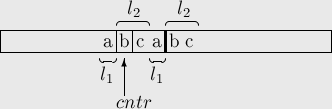
\includegraphics[scale=0.5]{11.png}

Here by $l_1$ and $l_2$ denotes the length of the two pieces of the tandem repeat: $l_1$ - Is the length of the tandem repeat to the position $cntr-1$ And $l_2$ - The length of a tandem repeat of $cntr$ before the end of half a tandem repeat. Thus, the $l_1 + l_2 + l_1 + l_2$ - The length of the tandem repeat.

Taking a look at this picture, you can see that \textbf{a necessary and sufficient} condition for a centered position $cntr$ is the length of tandem repeat $2 l = 2 (l_1 + l_2) = 2 (length (u) - cntr)$, Is the following condition:

Let $k_1$ - This is the largest number such that $k_1$ characters before your $cntr$ coincide with the last $k_1$ character string $u$ :
$u[cntr-k_{1}\ldots cntr-1]==u[length(u)-k_{1}\ldots length(u)-1]$

Let $k_2$ - This is the largest number such that $k_2$ characters, starting at position $cntr$ Coincide with the first $k_2$ character string $v$ :
$u[cntr\ldots cntr+k_{2}-1]==v[0\ldots k_{2}-1]$

Then it must be true:
$\begin{cases}
l_{1}\leq k_{1}\\
l_{2}\leq k_{2}
\end{cases}$

This criterion can be \textbf{reformulated} in this way. Fix a specific value $cntr$ Then:

All tandem repeats, which we now discover, have long $2 l = 2 (length (u) - cntr)$.
However, these tandem repeats may be \textbf{several:} it all depends on the choice of strips of $l_1$ and $l_2 = l - l_1$.

We find $k_1$ and $k_2$ As described above.
Then will be the appropriate tandem repeats for which the lengths of pieces $l_1$ and $l_2$ satisfy the following conditions:
$\begin{cases}
l_{1}+l_{2}=l=length(u)-cntr\\
l_{1}\leq k_{1}\\
l_{2}\leq k_{2}
\end{cases}$

Algorithm for finding the lengths $k_1$ and $k_2$
So the whole problem is reduced to the rapid calculation of long $k_1$ and $k_2$ for each value $cntr$.

We recall the definition:

$k_1$ - The maximum non-negative integer for which complete
$u[cntr-k_{1}\ldots cntr-1]==u[length(u)-k_{1}\ldots length(u)-1]$

$k_2$ - The maximum non-negative integer for which complete
$u[cntr\ldots cntr+k_{2}-1]==v[0\ldots k_{2}-1]$

On both of these requests can be responsible for $O (1)$ Using \textbf{algorithm for finding the Z-functions} :

To quickly find the values $k_1$ pre-calculate the Z-function for the line $\overline {u}$ (i.e. lines $u$ Written out in reverse order).
Then the value of $k_1$ for a specific $cntr$ is simply equal to the corresponding value of the array Z-function.

To quickly find the values $k_2$ pre-calculate the Z-function for the line $v + \# + u$ (i.e. lines $u$ Assigned to the line $v$ a separator character).
Again, the value $k_2$ for a specific $cntr$ should be easy to take from the corresponding element Z-function.

Find the right tandem repeats
Up to this point we have only worked with the left tandem repeats.

To search for the right tandem repeats, act the same way: we define the center $cntr$ as the character corresponding to the last character of a tandem repeat, who got into the first row.

Then the length $k_1$ will be determined as the number of characters to the position $cntr$ inclusive, coinciding with the last character $u$. Length $k_2$ will be defined as the maximum number of characters from the $cntr +1$ Coinciding with the first character $v$.

So, for a quick $k_1$ and $k_2$ it will be necessary to calculate in advance Z-function for strings $\overline {u} + \# + \overline {v}$ and $v$ respectively. After that, going through a particular value $cntr$, We are on the same criteria will be finding all the right tandem repeats.

Asymptotics
Asmiptotika algorithm Maine Lorenz will thus $O (n \log n)$ : Because this algorithm is the algorithm of "divide-and-conquer", each of which works recursively run in a time linear in the length of the string: for four strings in linear time sought their Z-function, and then moves the value $cntr$ and lists all of the detected tandem repeats.

Tandem repeats are found by the algorithm in the Maine-Lorentz form of original \textbf{groups} of fours $(Cntr, l, k_1, k_2)$, Each of which represents a group of tandem repeats of length $l$, The center of $cntr$ and with all sorts of strips of $l_1$ and $l_2$ Satisfying the conditions:

$\begin{cases}
l_{1}+l_{2}=l\\
l_{1}\leq k_{1}\\
l_{2}\leq k_{2}
\end{cases}$

\subsection{ Implementation }

We present implementation of the algorithm Maine Lorenzo, who for the time $O (n \log n)$ find all tandem repeats this line in a compressed form (as a group described by four numbers).

To demonstrate the tandem repeats found in the time $O (n ^ 2)$ "Decompress" and displayed separately. This conclusion is in solving real-world problems can easily be replaced by some other, more effective actions, for example, to search for naidlinneyshego tandem repeat, or count the number of tandem repeats.

\begin{verbatim}
vector < int > z_function(const string & s){
    int n =(int)s. length() ;
    vector < int > z(n);
    for(int i = 1, l = 0, r = 0 ; i < n ; ++ i){
        if(i <= r )
            z[i]= min(r - i + 1, z[i - l ]);
        while(i + z[i]< n && s[z[i]] == s[i + z[i]] )
            ++ z[i];
        if(i + z[i]- 1 > r )
            l = i,  r = i + z[i]- 1 ;
    }
    return z ;
}
 
void output_tandem(const string & s, int shift, bool left, int cntr, int l, int l1, int l2){
    int pos ;
    if(left )
        pos = cntr - l1 ;
    else
        pos = cntr - l1 - l2 - l1 + 1 ;
    cout << "[" << shift + pos << ".." << shift + pos + 2 * l - 1 << "] = " << s. substr(pos, 2 * l)<< endl ;
}
 
void output_tandems(const string & s, int shift, bool left, int cntr, int l, int k1, int k2){
    for(int l1 = 1 ; l1 <= l ; ++ l1){
        if(left && l1 == l) break ;
        if(l1 <= k1 && l - l1 <= k2 )
            output_tandem(s, shift, left, cntr, l, l1, l - l1);
    }
}
 
inline int get_z(const vector < int > & z, int i){
    return 0 <= i && i <(int)z. size() ? z[i]: 0 ;
}
 
void find_tandems(string s, int shift = 0){
    int n =(int)s. length() ;
    if(n == 1) return ;
 
    int nu = n / 2,  nv = n - nu ;
    string u = s. substr(0, nu ),
        v = s. substr(nu);
    string ru = string(u. rbegin(), u. rend() ),
        rv = string(v. rbegin(), v. rend());
 
    find_tandems(u, shift);
    find_tandems(v, shift + nu);
 
    vector < int > z1 = z_function(ru ),
        z2 = z_function(v + '#' + u ),
        z3 = z_function(ru + '#' + rv ),
        z4 = z_function(v);
    for(int cntr = 0 ; cntr < n ; ++ cntr){
        int l, k1, k2 ;
        if(cntr < nu){
            l = nu - cntr ;
            k1 = get_z(z1, nu - cntr);
            k2 = get_z(z2, nv + 1 + cntr);
        }
        else {
            l = cntr - nu + 1 ;
            k1 = get_z(z3, nu + 1 + nv - 1 -(cntr - nu)) ;
            k2 = get_z(z4,(cntr - nu)+ 1);
        }
        if(k1 + k2 >= l )
            output_tandems(s, shift, cntr < nu, cntr, l, k1, k2);
    }
} 
\end{verbatim}
\subsection{ Literature }

Michael Main, Richard J. Lorentz. \textbf{An O (n log n) Algorithm for Finding All Repetitions in a String} [1982]
Bill Smyth. \textbf{Computing Patterns in Strings} [2003]
Bill Smith. \textbf{Methods and calculation algorithms on strings} [2006]

